\documentclass[11pt,a4paper,oneside]{report}             % Single-side
%\documentclass[11pt,a4paper,twoside,openright]{report}  % Duplex

%\PassOptionsToPackage{chapternumber=Huordinal}{magyar.ldf}
\usepackage{t1enc}
\usepackage[latin2]{inputenc}
\usepackage{amsmath}
\usepackage{amssymb}
\usepackage{enumerate}
\usepackage[thmmarks]{ntheorem}
\usepackage{graphics}
\usepackage{epsfig}
\usepackage{listings}
\usepackage{color}
%\usepackage{fancyhdr}
\usepackage{lastpage}
\usepackage{anysize}
\usepackage[magyar]{babel}
\usepackage{sectsty}
\usepackage{setspace}  % Ettol a tablazatok, abrak, labjegyzetek maradnak 1-es sorkozzel!
\usepackage[hang]{caption}
\usepackage{hyperref}

%--------------------------------------------------------------------------------------
% Main variables
%--------------------------------------------------------------------------------------
\newcommand{\vikszerzo}{B�dis-Szomor� Andr�s}
\newcommand{\vikkonzulens}{dr.~Konzulens Elem�r}
\newcommand{\vikcim}{Elektronikus terel�k}
\newcommand{\viktanszek}{M�r�stechnika �s Inform�ci�s Rendszerek Tansz�k}
\newcommand{\vikdoktipus}{Diplomaterv}
\newcommand{\vikdepartmentr}{B�dis-Szomor� Andr�s}

%--------------------------------------------------------------------------------------
% Page layout setup
%--------------------------------------------------------------------------------------
% we need to redefine the pagestyle plain
% another possibility is to use the body of this command without \fancypagestyle
% and use \pagestyle{fancy} but in that case the special pages
% (like the ToC, the References, and the Chapter pages)remain in plane style

\pagestyle{plain}
%\setlength{\parindent}{0pt} % �ttekinthet�bb, angol nyelv� dokumentumokban jellemz�
%\setlength{\parskip}{8pt plus 3pt minus 3pt} % �ttekinthet�bb, angol nyelv� dokumentumokban jellemz�
\setlength{\parindent}{12pt} % magyar nyelv� dokumentumokban jellemz�
\setlength{\parskip}{0pt}    % magyar nyelv� dokumentumokban jellemz�

\marginsize{35mm}{25mm}{15mm}{15mm} % anysize package
\setcounter{secnumdepth}{0}
\sectionfont{\large\upshape\bfseries}
\setcounter{secnumdepth}{2}
\singlespacing
\frenchspacing

%--------------------------------------------------------------------------------------
%	Setup hyperref package
%--------------------------------------------------------------------------------------
\hypersetup{
    bookmarks=true,            % show bookmarks bar?
    unicode=false,             % non-Latin characters in Acrobat�s bookmarks
    pdftitle={\vikcim},        % title
    pdfauthor={\vikszerzo},    % author
    pdfsubject={\vikdoktipus}, % subject of the document
    pdfcreator={\vikszerzo},   % creator of the document
    pdfproducer={Producer},    % producer of the document
    pdfkeywords={keywords},    % list of keywords
    pdfnewwindow=true,         % links in new window
    colorlinks=true,           % false: boxed links; true: colored links
    linkcolor=black,           % color of internal links
    citecolor=black,           % color of links to bibliography
    filecolor=black,           % color of file links
    urlcolor=black             % color of external links
}

%--------------------------------------------------------------------------------------
% Set up listings
%--------------------------------------------------------------------------------------
\lstset{
	basicstyle=\scriptsize\ttfamily, % print whole listing small
	keywordstyle=\color{black}\bfseries\underbar, % underlined bold black keywords
	identifierstyle=, 					% nothing happens
	commentstyle=\color{white}, % white comments
	stringstyle=\scriptsize\sffamily, 			% typewriter type for strings
	showstringspaces=false,     % no special string spaces
	aboveskip=3pt,
	belowskip=3pt,
	columns=fixed,
	backgroundcolor=\color{lightgray},
} 		
\def\lstlistingname{lista}	

%--------------------------------------------------------------------------------------
%	Some new commands and declarations
%--------------------------------------------------------------------------------------
\newcommand{\code}[1]{{\upshape\ttfamily\scriptsize\indent #1}}

% define references
\newcommand{\figref}[1]{\ref{fig:#1}.}
\renewcommand{\eqref}[1]{(\ref{eq:#1})}
\newcommand{\listref}[1]{\ref{listing:#1}.}
\newcommand{\sectref}[1]{\ref{sect:#1}}
\newcommand{\tabref}[1]{\ref{tab:#1}.}

\DeclareMathOperator*{\argmax}{arg\,max}
%\DeclareMathOperator*[1]{\floor}{arg\,max}
\DeclareMathOperator{\sign}{sgn}
\DeclareMathOperator{\rot}{rot}
\definecolor{lightgray}{rgb}{0.95,0.95,0.95}

\author{\vikszerzo}
\title{\viktitle}
\includeonly{
	guideline,%
	project,%
	titlepage,%
	declaration,%
	abstract,%
	introduction,%
	chapter1,%
	chapter2,%
	chapter3,%
	acknowledgement,%
	appendices,%
}
%--------------------------------------------------------------------------------------
%	Setup captions
%--------------------------------------------------------------------------------------
\captionsetup[figure]{
%labelsep=none,
%font={footnotesize,it},
%justification=justified,
width=.75\textwidth,
aboveskip=10pt}

\renewcommand{\captionlabelfont}{\small\bf}
\renewcommand{\captionfont}{\footnotesize\it}

%--------------------------------------------------------------------------------------
% Table of contents and the main text
%--------------------------------------------------------------------------------------
\begin{document}
\singlespacing
%--------------------------------------------------------------------------------------
% Rovid formai es tartalmi tajekoztato
%--------------------------------------------------------------------------------------

\footnotesize
\begin{center}
\large
\textbf{\Large �ltal�nos inform�ci�k, a diplomaterv szerkezete}\\
\end{center}

A diplomaterv szerkezete a BME Villamosm�rn�ki �s Informatikai Kar�n:
\begin{enumerate}
\item	Diplomaterv feladatki�r�s
\item	C�moldal
\item	Tartalomjegyz�k
\item	A diplomatervez� nyilatkozata az �n�ll� munk�r�l �s az elektronikus adatok kezel�s�r�l
\item	Tartalmi �sszefoglal� magyarul �s angolul
\item	Bevezet�s: a feladat �rtelmez�se, a tervez�s c�lja, a feladat indokolts�ga, a diplomaterv fel�p�t�s�nek r�vid �sszefoglal�sa
\item	A feladatki�r�s pontos�t�sa �s r�szletes elemz�se
\item	El�zm�nyek (irodalomkutat�s, hasonl� alkot�sok), az ezekb�l levonhat� k�vetkeztet�sek
\item	A tervez�s r�szletes le�r�sa, a d�nt�si lehet�s�gek �rt�kel�se �s a v�lasztott megold�sok indokl�sa
\item	A megtervezett m�szaki alkot�s �rt�kel�se, kritikai elemz�se, tov�bbfejleszt�si lehet�s�gek
\item	Esetleges k�sz�netnyilv�n�t�sok
\item	R�szletes �s pontos irodalomjegyz�k
\item	F�ggel�k(ek)
\end{enumerate}

Felhaszn�lhat� a k�vetkez� oldalt�l kezd�d� \LaTeX-Diplomaterv sablon dokumentum tartalma. 

A diplomaterv szabv�nyos m�ret� A4-es lapokra ker�lj�n. Az oldalak t�k�rmarg�val k�sz�ljenek (mindenhol 2.5cm, baloldalon 1cm-es k�t�ssel). Az alap�rtelmezett bet�k�szlet a 12 pontos Times New Roman, m�sfeles sork�zzel.

Minden oldalon - az els� n�gy szerkezeti elem kiv�tel�vel - szerepelnie kell az oldalsz�mnak.

A fejezeteket decim�lis beoszt�ssal kell ell�tni. Az �br�kat a megfelel� helyre be kell illeszteni, fejezetenk�nt decim�lis sz�mmal �s kifejez� c�mmel kell ell�tni. A fejezeteket decim�lis al�oszt�ssal sz�mozzuk, maxim�lisan 3 al�oszt�s m�lys�gben (pl. 2.3.4.1.). Az �br�kat, t�bl�zatokat �s k�pleteket c�lszer� fejezetenk�nt k�l�n sz�mozni (pl. 2.4. �bra, 4.2 t�bl�zat vagy k�pletn�l (3.2)). A fejezetc�meket igaz�tsuk balra, a norm�l sz�vegn�l viszont haszn�ljunk sorkiegyenl�t�st. Az �br�kat, t�bl�zatokat �s a hozz�juk tartoz� c�met igaz�tsuk k�z�pre. A c�m a jel�lt r�sz alatt helyezkedjen el.

A k�peket lehet�leg rajzol� programmal k�sz�ts�k el, az egyenleteket egyenlet-szerkeszt� seg�ts�g�vel �rj�k le (A \LaTeX~ehhez k�zenfekv� megold�sokat ny�jt).

Az irodalomjegyz�k sz�vegk�zi hivatkoz�sa t�rt�nhet a Harvard-rendszerben (a szerz� �s az �vsz�m megad�s�val) vagy sorsz�mozva. A teljes lista n�vsor szerinti sorrendben a sz�veg v�g�n szerepeljen (sorsz�mozott irodalmi hivatkoz�sok eset�n hivatkoz�si sorrendben). A szakirodalmi forr�sok c�meit azonban mindig az eredeti nyelven kell megadni, esetleg z�r�jelben a ford�t�ssal. A list�ban szerepl� valamennyi publik�ci�ra hivatkozni kell a sz�vegben (a \LaTeX-sablon a Bib\TeX~seg�ts�g�vel mindezt automatikusan kezeli). Minden publik�ci� a szerz�k ut�n a k�vetkez� adatok szerepelnek: foly�irat cikkekn�l a pontos c�m, a foly�irat c�me, �vfolyam, sz�m, oldalsz�m t�l-ig. A foly�irat c�meket csak akkor r�vid�ts�k, ha azok nagyon k�zismertek vagy nagyon hossz�ak. Internet hivatkoz�sok megad�sakor fontos, hogy az el�r�si �t el�tt megadjuk az oldal tulajdonos�t �s tartalm�t (mivel a link egy id� ut�n ak�r el�rhetetlenn� is v�lhat), valamint az el�r�s id�pontj�t.

\vspace{5mm}
Fontos:
\begin{itemize}
	\item A szakdolgozat k�sz�t� / diplomatervez� nyilatkozata (a jelen sablonban szerepl� sz�vegtartalommal) k�telez� el��r�s Karunkon ennek hi�ny�ban a szakdolgozat/diplomaterv nem b�r�lhat� �s nem v�dhet� !
	\item Mind a dolgozat, mind a mell�klet maxim�lisan 15 MB m�ret� lehet !
\end{itemize}

\vspace{5mm}
\begin{center}
J� munk�t, sikeres szakdolgozat k�sz�t�st ill. diplomatervez�st k�v�nunk !
\end{center}

\normalsize

%--------------------------------------------------------------------------------------
% Feladatkiiras (a tanszeken atveheto, kinyomtatott valtozat)
%--------------------------------------------------------------------------------------
\clearpage
\begin{center}
\large
\textbf{FELADATKI�R�S}\\
\end{center}

A feladatki�r�st a tansz�ki adminisztr�ci�ban lehet �tvenni, �s a leadott munk�ba eredeti, tansz�ki pecs�ttel ell�tott �s a tansz�kvezet� �ltal al��rt lapot kell belef�zni (ezen oldal \emph{helyett}, ez az oldal csak �tmutat�s). Az elektronikusan felt�lt�tt dolgozatban m�r nem kell beleszerkeszteni ezt a feladatki�r�st.





\pagenumbering{arabic}
\onehalfspacing
%--------------------------------------------------------------------------------------
%	The title page
%--------------------------------------------------------------------------------------
\begin{titlepage}
\begin{center}

\includegraphics[width=60mm,keepaspectratio]{figures/BMElogo.png}\\
\vspace{0.3cm}
\textbf{Budapesti M�szaki �s Gazdas�gtudom�nyi Egyetem}\\
\textmd{Villamosm�rn�ki �s Informatikai Kar}\\
\textmd{\viktanszek}\\[5cm]

\vspace{0.4cm}
{\huge \bfseries \vikcim}\\[0.8cm]
\vspace{0.5cm}
\textsc{\Large \vikdoktipus}\\[4cm]

\begin{tabular}{cc}
 \makebox[7cm]{\emph{K�sz�tette}} & \makebox[7cm]{\emph{Konzulens}} \\
 \makebox[7cm]{\vikszerzo} & \makebox[7cm]{\vikkonzulens}
\end{tabular}

\vfill
{\large \today}
\end{center}
\end{titlepage}



\tableofcontents\vfill
%--------------------------------------------------------------------------------------
% Nyilatkozat
%--------------------------------------------------------------------------------------
\begin{center}
\large
\textbf{HALLGAT�I NYILATKOZAT}\\
\end{center}

Alul�rott \emph{\vikszerzo}, szigorl� hallgat� kijelentem, hogy ezt a diplomatervet meg nem engedett seg�ts�g n�lk�l, saj�t magam k�sz�tettem, csak a megadott forr�sokat (szakirodalom, eszk�z�k stb.) haszn�ltam fel. Minden olyan r�szt, melyet sz� szerint, vagy azonos �rtelemben, de �tfogalmazva m�s forr�sb�l �tvettem, egy�rtelm�en, a forr�s megad�s�val megjel�ltem.

Hozz�j�rulok, hogy a jelen munk�m alapadatait (szerz�(k), c�m, angol �s magyar nyelv� tartalmi kivonat, k�sz�t�s �ve, konzulens(ek) neve) a BME VIK nyilv�nosan hozz�f�rhet� elektronikus form�ban, a munka teljes sz�veg�t pedig az egyetem bels� h�l�zat�n kereszt�l (vagy autentik�lt felhaszn�l�k sz�m�ra) k�zz�tegye. Kijelentem, hogy a beny�jtott munka �s annak elektronikus verzi�ja megegyezik. D�k�ni enged�llyel titkos�tott diplomatervek eset�n a dolgozat sz�vege csak 3 �v eltelte ut�n v�lik hozz�f�rhet�v�.

\begin{flushleft}
\vspace*{1cm}
Budapest, \today
\end{flushleft}

\begin{flushright}
 \vspace*{1cm}
 \makebox[7cm]{\rule{6cm}{.4pt}}\\
 \makebox[7cm]{\emph{\vikszerzo}}\\
 \makebox[7cm]{hallgat�}
\end{flushright}
\thispagestyle{empty}

\vfill
\clearpage
\thispagestyle{empty} % an empty page


%----------------------------------------------------------------------------
% Abstract in hungarian
%----------------------------------------------------------------------------
\chapter*{Kivonat}\addcontentsline{toc}{chapter}{Kivonat}
 A mobil robotok manaps�g egyre ink�bb felt�rekv�ben vannak. M�r nem csak az ipar fedezi fel �ket, hanem lassan a mindennapi �let�nk r�sz�v� v�lnak. Azonban m�g rengeteg elm�leti �s gyakorlati k�rd�s v�r megold�sra, hogy az ilyen robotokkal rendszeresen tal�lkozzunk. A mobil robotika egyik legalapvet�bb k�rd�se az akad�lyok jelenl�t�ben t�rt�n� mozg�stervez�s �s mozg�sv�grehajt�s. A dolgozatban ezt a k�rd�sk�rt j�rjuk k�r�l, foglalkozunk a glob�lis �s lok�lis geometriai p�lyatervez�ssel, p�lyamenti sebess�gprofil kialak�t�s�val, valamint p�lyak�vet� szab�lyoz�ssal. Ezeket k�t, s�kban mozg�, kerekeken gurul� robotmodellre alkalmazzuk, mint szimul�lt, mint val�s k�rnyezetben.

A dolgozatban bemutatjuk a leggyakrabban haszn�lt p�lyatervez�si algoritmusokat, �s az ezekhez kapcsol�d� el�ny�ket �s probl�m�kat. K�l�n kit�r�nk az �ltalunk vizsg�lt (differenci�lis �s aut�szer�) robotmodellekn�l felmer�l� kinematikai korl�toz�sokra, �s ezek hat�saira a p�lyatervez�sben. Egy approxim�ci�s p�lyatervez�si megk�zel�t�st mutatunk be a dolgozatunkban, amely egy glob�lis �s egy lok�lis tervez� algoritmus egy�ttes haszn�lat�n alapszik.

Az �ltalunk alkalmazott RTR (Rotate-Translate-Rotate) glob�lis tervez� a szakirodalomb�l j�l ismert RRT (Rapidly Exploring Random Trees) elj�r�son alapul. Az RTR l�nyege, hogy a kiindul�si �s a c�l konfigur�ci�b�l k�t topol�giai f�t �p�t, �s amennyiben ezek el�rik egym�st, a keresett p�lya k�nnyed�n el��ll�that�. A p�lya forg�sokb�l (R) �s transzl�ci�s mozg�sokb�l (T) �ll, �gy differenci�lis robotok sz�m�ra k�zvetlen�l is v�grehajthat� p�ly�t eredm�nyez. Tov�bbi l�nyeges tulajdons�ga, hogy figyelembe veszi a robot pontos alakj�t. Ez hat�kony tervez�st tesz lehet�v� sz�k folyos�kat tartalmaz� k�rnyezet eset�n is, szemben az elterjedtebb, a robot alakj�t k�rrel helyettes�t� m�dszerekkel.

A megtervezett geometriai p�lya m�g nem tartalmaz inform�ci�t a mozg�s id�param�terez�s�re (a robot sebess�g�re, gyorsul�s�ra vagy sz�gsebess�g�re) n�zve. Ez�rt bemutatunk egy �ltalunk kifejlesztett algoritmust a p�lyamenti sebess�gprofil meghat�roz�s�ra. Ezt a profilt a robot maxim�lis sebess�ge, maxim�lis gyorsul�sa, maxim�lis sz�gsebess�ge �s a robot kerekeinek maxim�lis gyorsul�sa alapj�n sz�moljuk ki. Az �gy kialakul� p�ly�t ezut�n �jramintav�telezz�k, hogy id�ben egyenletes mintav�tel� p�lya �lljon rendelkez�sre p�lyak�vet� szab�lyoz�s sz�m�ra.

A p�lyak�vet� algoritmus a robot p�lyamenti sebess�g�t �s a sz�gsebess�g�t f�ggetlen�l szab�lyozza. A sz�tcsatolt rendszer sebess�g �s sz�gsebess�g beavatkoz� jeleit a robot kinematikai egyenletei alapj�n �talak�tjuk ker�ksebess�g beavatkoz� jelekre. A sebess�g-szab�lyoz�si k�r a robot t�nyleges poz�ci�ja alapj�n egy PD szab�lyoz�n kereszt�l korrig�lja az el��rt sebess�gprofilt. A sz�gsebess�g-szab�lyoz�s egy mozg�s k�zbeni orient�ci� korrekci�t hajt v�gre, melynek alapj�t a robot k�s�bbi el��rt poz�ci�i k�pezik.

A fent le�rt algoritmusokat differenci�lis robotmodellt felt�telezve alak�tottuk ki. A dolgozatban bemutatjuk azokat a m�dos�t�sokat, illetve kieg�sz�t�seket, amelyek lehet�v� teszik a p�lyatervez�st �s k�vet�st aut�szer� (korm�nyzott) robotok eset�ben is. Ennek keret�ben bemutatjuk a C*CS lok�lis p�lyatervez� algoritmust, amely az RTR algoritmussal egy�tt alkalmazva olyan p�ly�t eredm�nyez, amely figyelembe veszi az aut� minim�lis fordul�si sugar�t.

Az algoritmusokat a V-REP robotszimul�ci�s k�rnyezetben implement�ltuk �s tesztelt�k, majd m�k�d�s�ket k�t val�s roboton is vizsg�ltuk. 
\vfill

%----------------------------------------------------------------------------
% Abstract in english
%----------------------------------------------------------------------------
\chapter*{Abstract}\addcontentsline{toc}{chapter}{Abstract}


\vfill


%----------------------------------------------------------------------------
\chapter*{Bevezet�}\addcontentsline{toc}{chapter}{Bevezet�}
%----------------------------------------------------------------------------

A dolgozatom c�lja, hogy az elm�letben kidolgozott p�lyak�vet�si �s mozg�sir�ny�t�si m�dszereket gyakorlatban is kipr�b�ljam. Ehhez term�szetesen a p�lyatervez�s, mozg�sk�vet�s elm�leti ismereteire, valamint a gyakorlati tapasztalatok alapj�n a kidolgozott algoritmusok m�dos�t�s�ra is sz�ks�g van. A diplomatervem ezt a folyamatot k�veti v�gig.

A dolgozat elej�n r�viden ismertetj�k a p�lyatervez�shez �s p�lyak�vet�shez sz�ks�ges alapvet� fogalmakat. Ezenk�v�l bemutatom a munk�m sor�n alkalmazott kinematikai robotmodellt, �s az alapvet� p�lyatervez�si m�dszerek csoportos�t�sait. 

A m�sodik fejezetben r�t�r�nk egy glob�lis p�lyatervez�, az RTR algoritmus t�rgyal�s�ra. Az RTR algoritmus meg�rt�s�hez sz�ks�ges az �gynevezett RRT elj�r�st bevezetni, amelyet p�lyatervez�si feladatokn�l igen gyakran alkalmaznak. Az RTR tervez� elm�leti t�rgyal�sa ut�n, ismertetem az implement�l�shoz kapcsol�d� gyakorlati probl�m�kat. Az implement�l�s  bemutat�sa ut�n a tervez� �ltal tervezett, konkr�t p�ly�kat vizsg�ljuk meg.

A p�lyatervez�shez kapcsol�dik az id�param�terez�s k�rd�se, amelyet a harmadik fejezetben t�rgyalunk. Az id�param�terez�s a p�lyatervez� �ltal tervezett p�ly�hoz sebess�ginform�ci�t rendel, a robot korl�toz�sait figyelembe v�ve. Az id�param�terez�s kimenete egy id�ben egyenletesen mintav�telezett p�lya, amelyet a p�lyak�vet� algoritmus haszn�l fel. Itt is konkr�t p�ld�n mutatjuk meg a megtervezett p�ly�hoz tartoz� sebess�g- �s gyorsul�sprofilokat.

A p�lyatervez�s ut�n �tt�r�nk a p�lyak�vet�s ismertet�s�re. A p�lyak�vet�s alapvet�en k�t geometriai primit�vvel dolgozik: egy helyben fordul�s �s p�lyak�vet�s. Ezeket t�rgyaljuk r�szletesen a negyedik fejezetben. A fejezet sor�n ismertetj�k a sebess�gszab�lyoz�st �s az orient�ci�szab�lyoz�st, valamint az ezekhez kapcsol�d� probl�m�kat. A fejezet v�g�n az algoritmus �ltal felhaszn�lt param�terek hat�sait vizsg�ljuk meg. 

V�g�l, az �t�dik fejezetben a p�lyatervez� �s mozg�sir�ny�t� algoritmusokat rendszerbe foglaljuk. Ehhez kapcsol�d�an r�viden eml�t�st tesz�nk egy m�sik p�lyatervez� elj�r�sr�l, a C*CS algoritmusr�l. Szint�n ebben a fejezetben mutatjuk be az �ltalam haszn�lt V-REP  robotszimul�tort, a szimul�ci�s eredm�nyeket, �s a szimul�torhoz kifejlesztett keretrendszert. A dolgozat v�g�n a val�s robotot ismertetj�k, k�l�n�sk�ppen a robot ir�ny�t�rendszer�t. Az �ltalam implement�lt algoritmusokat ebbe az ir�ny�t�programba kellett integr�lni. A dolgozat z�r�sak�nt a val�s roboton m�rt eredm�nyeket vizsg�ljuk meg.
%----------------------------------------------------------------------------
\chapter{Bevezet�s}
%----------------------------------------------------------------------------

%----------------------------------------------------------------------------
\section{Probl�mafelvet�s}
%----------------------------------------------------------------------------
A helyv�ltoztat�sra k�pes, �gynevezett mobil robotok eset�ben gyakran el�fordul� probl�ma, hogy robotnak a feladata v�grehajt�s�hoz el kell jutnia egy adott c�lpontba. Ehhez �nmag�nak kell az adott k�rnyezetben megterveznie a p�ly�t �s emberi beavatkoz�s n�lk�l kell sikeresen eljutnia a k�v�nt c�lpontba. A probl�ma nagys�grendileg nehezebb amikor a robot k�rnyezet�ben akad�lyok is tal�lhat�ak. 

\par
A mi c�lunk a p�lyatervez�si m�dszerek bemutat�sa, n�h�ny m�dszer implement�l�sa �s tesztel�se szimul�torban �s val�s robotokon is. A p�lyatervez�shez szorosan kapcsol� t�ma a mozg�sir�ny�t�s, amivel szint�n foglalkoznunk kell, hogy val�s k�rnyezetben t�nylegesen haszn�lhat� elj�r�sokat kapjunk.

%----------------------------------------------------------------------------
\section{P�lyatervez�s elm�lete}
%----------------------------------------------------------------------------
Az elm�lt id�szakban a p�lyatervez�ssel kapcsolatban igen sok kutat�s foglalkozott \cite{Latombe}. Ahhoz, hogy ezeket az algoritmusokat ismertess�k, be kell vezetn�nk n�h�ny alapvet� fogalmat. 

%----------------------------------------------------------------------------
\subsection{Alapvet� fogalmak}
%----------------------------------------------------------------------------
A p�lyatervez�s sor�n a robot pillanatnyi �llapot�t a \emph{konfigur�ci�j�val} �rhatjuk le. S�kban mozg� robotok eset�ben a konfigur�ci� a k�vetkez�ket tartalmazza \cite{Springer}:

\begin{align}
q &= (x,y,\theta),
\end{align}
ahol $q$ a robot konfigur�ci�ja, $x,y$ hat�rozza meg a robot poz�ci�j�t a s�kon �s $\theta$ hat�rozza meg a robot orient�ci�j�t.

Egy lehets�ges k�rnyezetben a robot �sszes �llapot�t, a \emph{konfigur�ci�s t�r} adja meg, amit $C$-vel jel�l�nk. A konfigur�ci�s t�r azon halmaz�t, amely eset�ben a robot a k�rnyezetben tal�lhat� akad�lyokkal nem �tk�zik, \emph{szabad (konfigur�ci�s) t�rnek} nevez�nk ($C_{free}$). E halmaz komplementere azokat a konfigur�ci�kat tartalmazza, amelyek eset�n a robot �tk�zne az akad�lyokkal ($C_{obs} = C \backslash C_{obs}$).

\par
A korl�toz�sok ismerete alapvet� fontoss�g� a p�lyatervez�s �s mozg�sir�ny�t�s sor�n. A k�rnyezetben elhelyezked� akad�lyokat \emph{glob�lis korl�toz�soknak} tekintj�k, a robothoz kapcsol�d� korl�toz�sokat pedig \emph{lok�lis korl�toz�soknak} \cite{Springer}. A lok�lis korl�toz�sokat a robot konfigur�ci�s v�ltoz�inak differenci�l egyenlet�vel �rhatjuk le, ez�rt gyakran nevezik �ket \emph{differenci�lis korl�toz�soknak} is. Differenci�lis korl�toz�sok vonatkozhatnak sebess�g (kinematikai) �s gyorsul�s mennyis�gre is (dinamikai korl�t). %TODO �gy j�?

\par
A mi dolgozatunkban kinematikai korl�toz�sokkal fogunk foglalkozni.

\par
Egy aut� eset�n mindenki sz�m�ra egy�rtelm�, hogy csak bizonyos �veken tudunk mozogni, egy adott konfigur�ci�b�l nem tudunk a konfigur�ci�s t�r b�rmely ir�ny�ba elmozdulni. Aut�n�l emiatt nem olyan egyszer� a p�rhuzamosan parkol�s. Azokat a robotokat, amelyek ehhez hasonl� korl�toz�sokkal rendelkeznek, \emph{anholonom rendszereknek} nevezz�k. Az anholonom korl�toz�sr�l akkor besz�l�nk, ha a korl�toz�s olyan differenci�l egyenlettel �rhat� le, amely nem integr�lhat�.

\par
Az �ltalunk vizsg�lt k�t robot t�pus, az \emph{aut�szer� robotok} �s a \emph{differenci�lis robotok} is anholonom rendszerek. Viszont l�teznek olyan robotok, amelyek nem rendelkeznek anholonom korl�toz�sokkal (holonom rendszerek), ilyenek p�ld�ul az omnidirekcion�lis robotok. Egy omnidirekcion�lis robot k�pes a t�r b�rmely ir�ny�ba elmozdulni.

%----------------------------------------------------------------------------
\subsubsection{Robotmodellek}
%----------------------------------------------------------------------------


%----------------------------------------------------------------------------
\subsection{Oszt�lyoz�s}
%----------------------------------------------------------------------------

%----------------------------------------------------------------------------
\subsubsection{Lok�lis m�dszerek}
%----------------------------------------------------------------------------
A topol�giai felt�tel defin�ci�ja:

%TODO a megfelel� heyleken k�ne space, illetve valahogy align egym�shoz k�pset
\begin{align}\label{eq:topologicalProp}
\forall \epsilon > 0, \exists \eta > 0, \forall q_{0},q_{1} \in C \\ \notag
d_{\mathcal{C}}(q_{0},q_{1}) < \eta \rightarrow d_{\mathcal{C}}\left(q_{0}, Steer(q_{0},q_{1})(\sigma)\right) < \epsilon \\ \notag
\forall \sigma \in [q,S]
\end{align}

%----------------------------------------------------------------------------
\subsubsection{Glob�lis m�dszerek}
%----------------------------------------------------------------------------

%----------------------------------------------------------------------------
\chapter{�tvonaltervez�s C*CS p�ly�kkal}
%----------------------------------------------------------------------------
A C*CS �s a $c\overline{c}S$ algoritmus Kiss Domokos munk�ja \cite{CCSTopologicalProp}. Az algoritmusok els�dlegesen aut�szer� robotok sz�m�ra terveznek p�ly�t, de az �gy tervezett p�lya egy differenci�lis robot sz�m�ra is v�grehajthat�. Feladatom az algoritmus implement�l�sa volt C++ nyelven, majd annak tesztel�se szimul�ci�s, illetve val�s k�rnyezetben.
A fejezetet az algoritmus ismertet�s�vel kezdem, majd kit�rek az implement�ci�s probl�m�kra, �s az el�rt eredm�nyekre is.

%----------------------------------------------------------------------------
\section{Reeds-Shepp lok�lis p�ly�k}
%----------------------------------------------------------------------------
Az anholonom rendszerek ir�ny�t�sa akad�lyokt�l mentes k�rnyezetben is egy igen bonyolult feladat. Sok esetben nem adhat� meg �ltal�nos algoritmus, csak n�h�ny speci�lis rendszer eset�n. Szerencs�re ilyen rendszerek k�z� tartoznak a differenci�lis robotok, az aut�szer� robotok, amelyek csak el�re mozoghatnak (Dubins aut�), �s azok, amelyek el�re �s h�tra is k�pesek mozogni.

\begin{figure}[H]
\centering
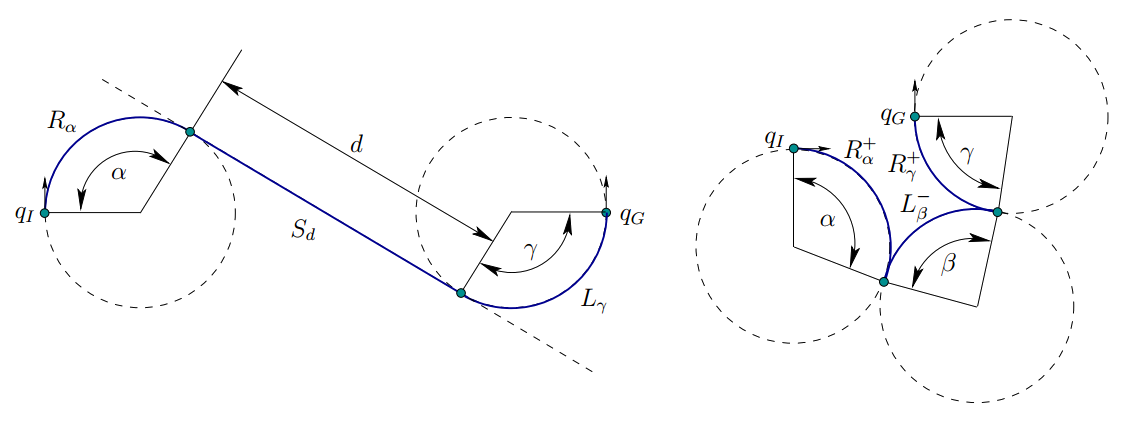
\includegraphics[width=130mm, keepaspectratio]{figures/dubins-reeds-shepp.png}
\caption{Dubins �s Reeds-Shepp megold�sok \cite{LaValle2}} 
\label{fig:reeds_shepp}
\end{figure}

Az ut�bbi t�pus� robotokat h�vjuk Reeds-Shepp aut�knak, melyekn�l bizony�tott, hogy b�rmely kezd�- �s c�lkonfigur�ci� k�zt a legr�videbb utat megtal�lhatjuk 48 lehets�ges megold�s k�z�l, amelyb�l kett� l�that� \aref{fig:reeds_shepp} �br�n. Ezek a lehets�ges megold�sok maximum �t egyenes vagy minim�lis sugar� k�r�v kombin�ci�j�b�l �llhatnak, �s a p�ly�k maximum k�t cs�csot tartalmazhatnak, azaz ennyiszer lehet ir�nyt v�ltoztatni a v�grehajt�s k�zben \cite{ReedsShepp}.

Mint l�that�, akad�lyokt�l mentes k�rnyezetben tal�lhatunk optim�lis �tvonalat, de ennek h�tr�nya, hogy mindig minim�lis sugar� p�ly�kat felt�telez, mely egy val�s esetben nem �letszer�, illetve a p�ly�k lehetnek igen bonyolultak is. Azonban ha elvetj�k az optimalit�s ig�ny�t -- amit egy�bk�nt is meg kell tenn�nk, ha egy glob�lis tervez� r�szek�nt alkalmazzuk a m�dszert -- akkor a lehets�ges megold�sokon jelent�s m�rt�kben egyszer�s�thet�nk.

%----------------------------------------------------------------------------
\section{C*CS lok�lis p�ly�k}\label{CCSlocal}
%----------------------------------------------------------------------------
A lok�lis tervez�k b�rmely kezd�- �s c�lkonfigur�ci� p�ros eset�n megold�st kell ny�jtsanak, de megfelel� koordin�ta-rendszer v�laszt�s�val egyszer�s�thet�nk a sz�m�t�sokon. Tegy�k fel, hogy egy ilyen v�laszt�s mellett ad�dott $q_{I} = (x_{I},y_{I},\theta_{I})$ kezd� �s $q_{G} = (0,0,0)$ c�lkonfigur�ci�. Ha eltekint�nk a minim�lis fordul�si sug�r korl�toz�s�t�l, �s feltessz�k, hogy $\theta_{I} \neq 0$, akkor k�nnyen bel�that�, hogy egy k�r �s egy egyenes seg�ts�g�vel el�rhet� a c�lkonfigur�ci�. El�sz�r egy �rint� k�r�n elfordulunk a $\tilde{q_{G}} = (\tilde{x_{G}},0,0)$ k�ztes c�lkonfigur�ci�ba, majd egy egyenes ment�n v�gighaladunk a c�lig. Az ehhez tartoz� k�r sugar�t a k�vetkez� egyenlet seg�ts�g�vel sz�m�thatjuk:
\begin{align}\label{eq:middleRadius}
\rho_{I,\tilde{G}} = \frac{y_{I}}{1 - \cos \theta_{I}}
\end{align}

Ha a kiad�d� sug�r kisebb, mint a minim�lisan megengedett ($|\rho_{I,\tilde{G}}| < \rho_{min}$), esetleg $\theta_{I} = 0$, akkor egy egyenes vagy egy k�r seg�ts�g�vel egy k�ztes kezd�konfigur�ci�ba ($\tilde{q_{I}} = (\tilde{x_{I}},\tilde{y_{I}},\tilde{\theta_{I}})$) kell eljutnunk, ahol biztos�tott, hogy $\tilde{\theta_{I}} \neq 0$ �s, hogy $\rho_{\tilde{I},\tilde{G}} \geq \rho_{min}$. Megjegyzend�, hogy az els� szakasz nem lehet egyenes, ha $\theta_{I} = 0$, $\theta_{I} = \pi$ vagy $|y_{I}| < 2\rho_{min}$. Bebizony�that� \cite{CCSTopologicalProp}, hogy $\tilde{q_I}$ k�ztes konfigur�ci�t v�gtelen sokf�lek�ppen megv�laszthatjuk.

Hogy egyszer�s�ts�k a jel�l�seket, a tov�bbiakban az egyenes szakaszokra $S$, a k�r�vekre pedig a $C$ bet�k seg�ts�g�vel hivatkozunk. Ezt felhaszn�lva bel�that�, hogy a c�lpontba egy $SCS$, vagy egy $CCS$ p�lya seg�ts�g�vel eljuthatunk. K�nnyen bel�that�, hogy ha egy k�r�v ($C$) sugar�val a v�gtelenbe tartunk, akkor a szakasz az egyeneshez tart. Az olyan speci�lis k�r�veket, amelyek sugara v�gtelen is lehet, $C^{*}$-gal jel�lj�k. Innen a m�dszer neve, a $C^{*}CS$.


%----------------------------------------------------------------------------
\section{C*CS approxim�ci�s m�dszer}
%----------------------------------------------------------------------------
Az �ltalam haszn�lt algoritmus egy approxim�ci�s m�dszert alkot, mely egy el�zetes glob�lis p�ly�t rekurz�v m�don felbont kisebb szakaszokra, majd ezekre pr�b�l illeszteni egy-egy fentebb bemutatott C*CS p�ly�t.\footnote{B�r a lok�lis tervez� algoritmus neve a C*CS, de a v�geredm�nyben kialakult p�lya �sszess�g�ben is k�r�k �s egyenesek kombin�ci�j�b�l �ll, �gy ez a n�v r�ragadt az approxim�ci�s m�dszerre is.} A v�geredm�ny�l elk�sz�lt, az algoritmus �ltal visszaadott p�lya aut�szer� robotokkal k�nnyed�n lek�vethet�, mivel els�dlegesen ezek sz�m�ra lett kialak�tva. Ennek ellen�re a megold�st term�szetesen egy differenci�lis robot is k�pes lek�vetni, mivel az nem rendelkezik korl�toz�ssal a fordul� k�r sugar�t illet�en.

\subsection{Glob�lis tervez�}
A sz�ks�ges el�zetes p�lya b�rmilyen glob�lis tervez� eredm�nye lehet. Els�dleges c�lja egy mank� ny�jt�sa a k�s�bbi tervez� sz�m�ra. A v�gs� megold�snak nem felt�tele, hogy az el�zetes p�lya ak�r egyetlen pontj�t is tartalmazza.

Mi erre a c�lra egy celladekompoz�ci�n alapul� algoritmust haszn�ltunk. Ez az elj�r�s a k�rnyezetet h�romsz�gekre bontja \cite{fade2d}, majd ezeknek a h�romsz�geknek az oldalfelez� pontjait �sszek�tve gr�fot alkot. Ebbe besz�rja a kezd�- �s c�lkonfigur�ci�t, majd ezeket �sszek�ti a legk�zelebb �ll� n�h�ny ponttal. Az �leket a pontok egym�st�l val� t�vols�g�val s�lyozzuk, majd ebben a gr�fban a Dijkstra-algoritmus \cite{BFS} seg�ts�g�vel megkeress�k a legr�videbb utat. Erre egy p�ld�t \aref{fig:ccs_triang} �br�n l�thatunk.

\begin{figure}
	\centering
	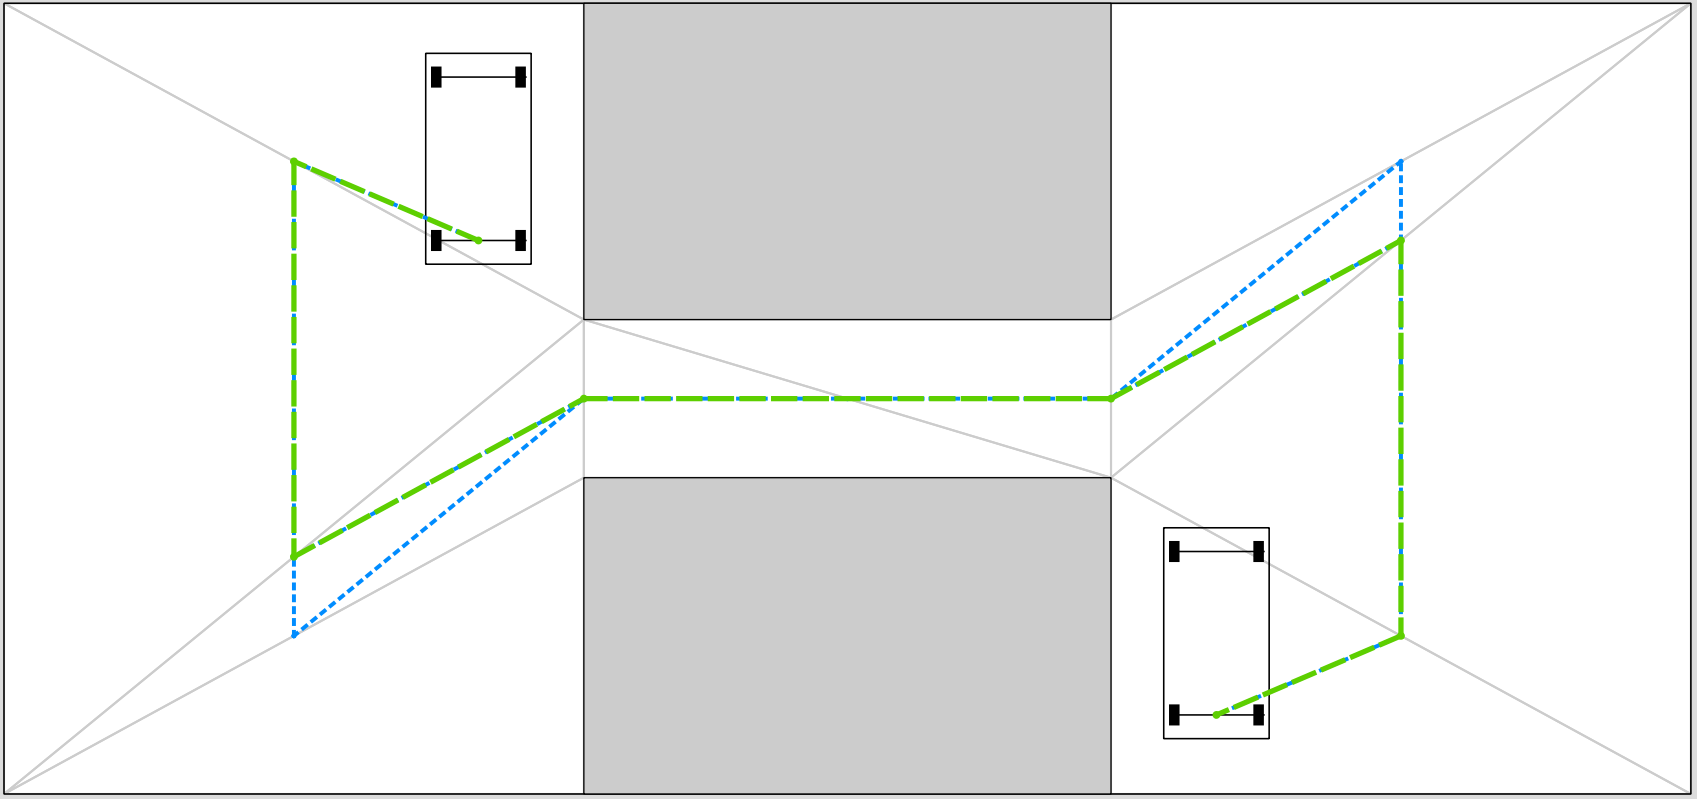
\includegraphics[width=130mm, keepaspectratio]{figures/ccs_prepath.png}
	\caption{El�zetes p�lya tervez�se, sz�rke h�romsz�gek a szabad t�r felbont�s�t, pontozott vonal a gr�fot, szaggatott vonal pedig az elk�sz�lt el�zetes p�ly�t jelzi} 
	\label{fig:ccs_triang}
\end{figure}

Ennek a megold�snak az el�nye, hogy nagyj�b�l a szabad ter�let k�zep�n alkot p�ly�t, �gy ha az aut� ezt k�veti, akkor b�rmilyen ir�ny� man�verez�sre lesz lehet�s�ge, ha a p�lya ezt megengedi. Tov�bbi el�nye, hogy ez egy kombinatorikus elj�r�s, �gy v�ges id�n bel�l k�pes megmondani, hogy l�tezik-e megold�s. Az elj�r�s egyik f� hib�ja, hogy a h�romsz�gel�s miatt csak soksz�gekkel le�rhat� akad�lyokkal k�pes dolgozni, �s m�g ebben a form�j�ban nem veszi figyelembe az aut� kiterjed�s�t. Ezen k�nnyen lehet seg�teni, ha figyelembe vessz�k az oldalfelez� pontok k�z�tti szakaszok t�vols�g�t az akad�lyokt�l, �s ha a p�lya- �s az akad�ly�l t�l k�zel vannak egym�shoz, akkor t�r�lj�k az �lt a gr�fb�l. Sajnos az elj�r�s egy�b negat�vumokkal is b�r, amir�l a fejezet v�g�n m�g sz�t ejtek.

\subsection{Lok�lis tervez� alkalmaz�sa}
Ha a glob�lis tervez� tudott visszaadni megold�st, akkor az algoritmus tov�bb folytat�dik a k�vetkez�k�ppen: Az el�zetes p�lya k�t konfigur�ci�j�t kiv�lasztjuk, �s a fentebb eml�tett C*CS p�ly�kat keres�nk k�zt�k. Az elj�r�s el�sz�r a p�lya k�t v�gpontja k�zt keres �tvonalat, ami egyszer� esetekben ak�r r�gt�n megold�sra is vezethet, felgyors�tva az algoritmus m�k�d�s�t. Ha ez a keres�s nem j�rt sikerrel, akkor az el�zetes p�ly�t megfelezi az algoritmus, �s az els� konfigur�ci�, valamint a f�lp�ly�hoz legk�zelebb es� sarokpontbeli konfigur�ci� k�zt keres megold�st. Ezt eg�szen addig ism�tli, m�g van k�ztes sarokpont a p�ly�ban. Ha elfogyott, tov�bbi pontokat illeszt a p�ly�ba.

Az el�z�ekben l�thattuk, hogy a C*CS v�gtelen sok megold�st ny�jt. Lok�lis esetben ez nem felt�tlen hasznos, de akad�lyok jelenl�t�ben m�r igen, mivel �gy sokkal nagyobb val�sz�n�s�ggel tal�lhatunk v�grehajthat� p�ly�t. Term�szetesen az �sszes megold�st nincs lehet�s�g�nk kipr�b�lni, �gy ezt a probl�m�t valamilyen mintav�telez� elj�r�ssal kell megoldanunk.

\begin{figure}[H]
\centering
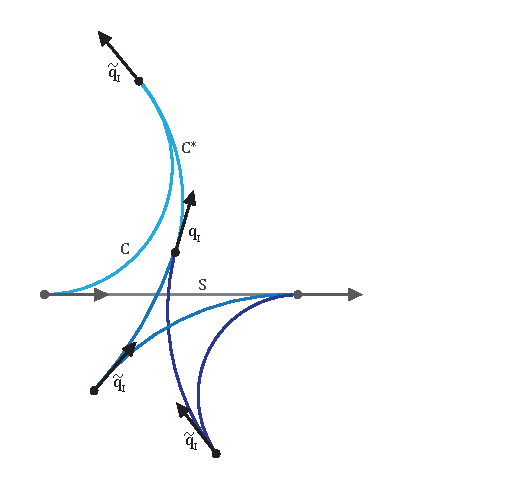
\includegraphics[width=75mm, keepaspectratio]{figures/CCS.pdf}
\caption{$q_{\tilde{I}}$ megv�laszt�sa } 
\label{fig:infCCS}
\end{figure}

A v�gtelen sok megold�st a $\tilde{q_{I}}$ kiv�laszt�s�nak szabads�ga okozza. Erre egy p�lda l�that� \aref{fig:infCCS} �br�n. Ez�rt az algoritmus �sszegy�jti azokat a konfigur�ci�kat, melyeket a $q_{I}$ konfigur�ci�b�l �tk�z�s n�lk�l el�rhet�nk. Ehhez a k�rnyezetet fel kell osszuk egys�gnyi t�vols�gokra, mivel �gy v�ges sok lehet�s�get kapunk. A kisz�m�t�s ideje term�szetesen f�gg a v�lasztott t�vols�gegys�gt�l �s a k�rnyezet m�ret�t�l. Az eredm�nyek azt mutatj�k, hogy a teljes algoritmus fut�s�nak ez a leghosszabb r�sze, ami nem meglep�, mivel a k�r�vek kisz�m�t�sa komplex m�velet, �s ezt egy adott pont eset�n a robot test�nek minden cs�cs�ra ki kell sz�moljuk, hogy �tk�z�st tudjunk detekt�lni. A m�velet hat�konys�g�n t�bb m�don lehet jav�tani, p�ld�ul nagyobb t�vols�gegys�g megv�laszt�s�val. M�sik jav�t�si lehet�s�g, ha el�re elk�sz�t�nk egy foglalts�gi m�trixot, ami megmondja az adott pont akad�lyon be�l van-e, �gy ezekre a pontokra nem kell a sz�m�t�st elv�gezni. Mivel az �gy kapott k�r�vek egy adott kezd�konfigur�ci�hoz tartoznak, tov�bbi gyors�t�sra ad lehet�s�get, ha az approxim�ci�s l�p�sben ink�bb a c�lkonfigur�ci� pontj�t mozgatjuk, �gy nem kell �jra �s �jra kisz�molni a k�r�ven el�rhet� sokas�got.

\begin{figure}[H]
\centering
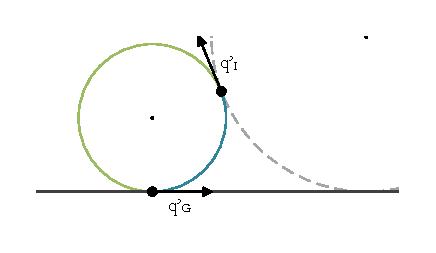
\includegraphics[width=90mm, keepaspectratio]{figures/CS.pdf}
\caption{K�z�ps� k�r�v sz�m�t�sa �rint� k�rrel} 
\label{fig:erintoKor}
\end{figure}

Az algoritmus tov�bbi r�sz�ben \aref{CCSlocal} pontban eml�tett m�don, a h�tral�v� k�r�v, �s egyenes szakasz kisz�m�t�sa a feladat. Egy ir�ny�tott k�r eset�n ez k�t lehets�ges p�ly�t jelent, amint az l�that� \aref{fig:erintoKor} �br�n. Ezek ut�n nem el�g csak a k�r�vek v�grehajthat�s�g�t ellen�rizn�nk, hanem meg kell n�zz�k ezt a h�tral�v� egyenes szakaszokra is. Ugyan a glob�lis p�lya tervez�sekor ellen�rizt�k ezeket, de az �rint� k�r�k keres�sekor nem volt felt�tel, hogy az �rint�si pontok ezeken a szakaszokon bel�l helyezkedjenek el.

V�g�l az �gy keletkez� v�grehajthat� p�ly�k sokas�ga k�z�l ki kell v�lasztanunk egyet. Ezt t�bbf�lek�ppen megtehetj�k. Tal�n a legk�zenfekv�bb a legr�videbb megold�s kikeres�se �s beilleszt�se az el�zetes p�ly�ba. Itt �rdemes megeml�teni, hogy a v�geredm�ny akkor fog igaz�n hasonl�tani a val�s�ghoz, ha lecs�kkentj�k a tolat�sok sz�m�t, mivel az emberek nagy t�bbs�ge nem szeret tolatva k�zlekedni. Hogy ezt megtehess�k, az algoritmus opcion�lisan elfogad egy s�lyt�nyez�t, mellyel a tolat� szakaszok ``hossz�t'' tudjuk megn�velni.

\begin{figure}[H]
\centering
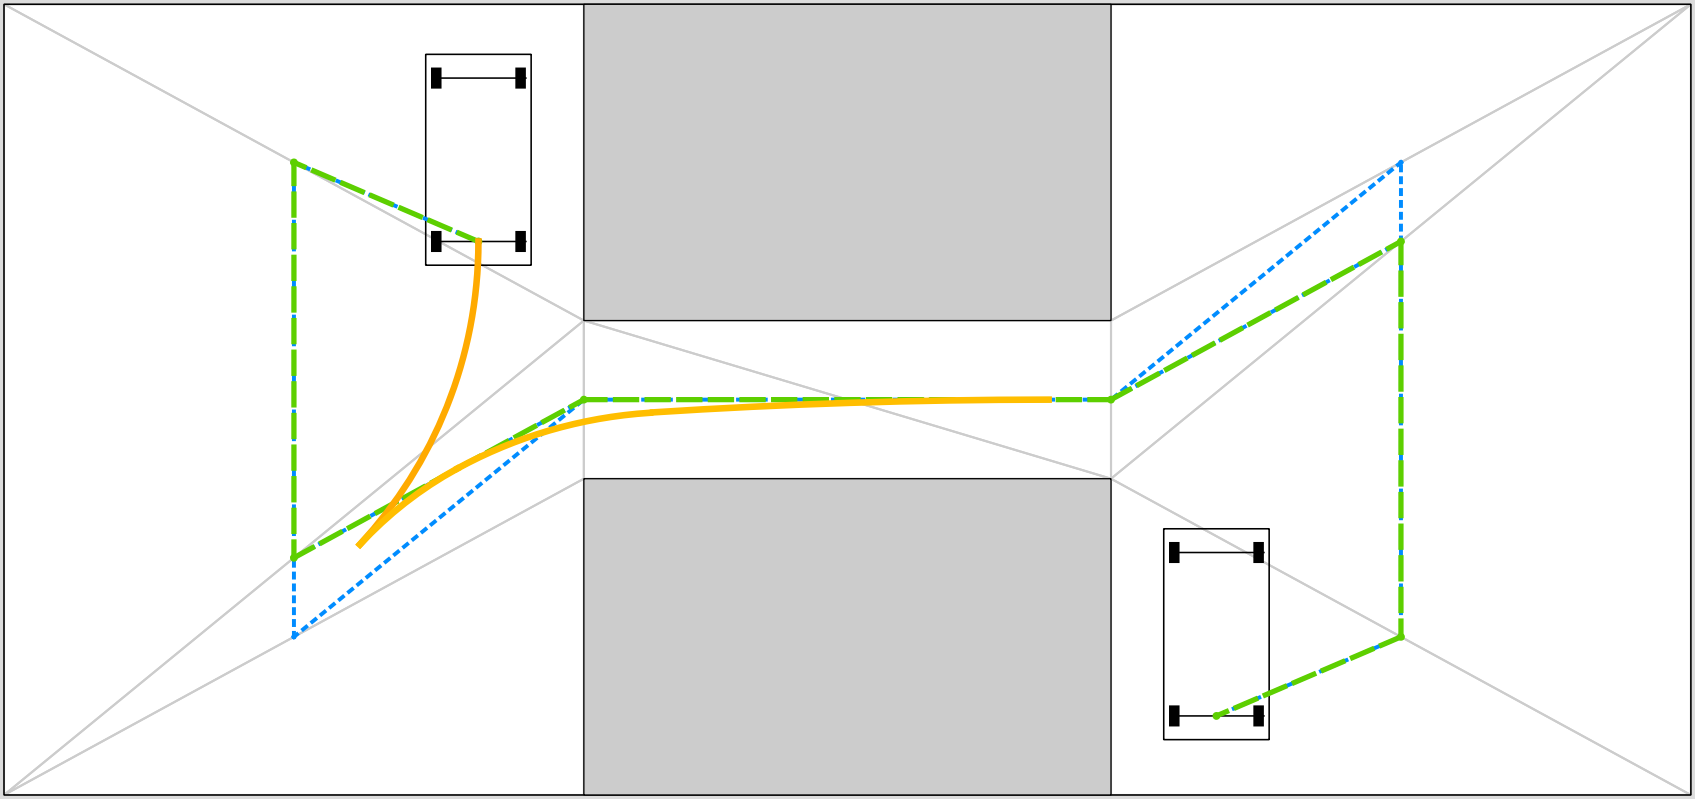
\includegraphics[width=130mm, keepaspectratio]{figures/ccs_middle.png}
\caption{A C*CS algoritmus m�k�d�s k�zben} 
\label{fig:CCSonline}
\end{figure}

%----------------------------------------------------------------------------
\section{ \texorpdfstring{\boldmath{$c\overline{c}S$}}{ccS} lok�lis tervez� algoritmus }
%----------------------------------------------------------------------------
Ha az el�z�ekben l�tottak nem vezetnek megold�sra, teh�t nincs olyan C*CS p�lya, mely v�grehajthat� lenne, akkor egy kisebb szakaszt kell v�lasztanunk a glob�lis p�ly�b�l. Ezt viszont nem tehetj�k meg v�gtelens�gig, mivel a glob�lis p�lya �ltal�ban egyenes szakaszok egy�ttes�b�l �ll. Ezek a szakaszok hat�rozz�k meg az $S$ szakasz egyenes�t, �gy tov�bb bontani nincs �rtelme, mert nem v�ltoztatja meg a tervezett p�ly�t. Ez�rt az �j konfigur�ci�kat a t�r�spontokban kell elhelyezni, viszont �nmag�ban ez m�g nem biztos�tja, hogy tal�lunk megold�st. Valahogy biztos�tanunk kell azt, hogy az algoritmusunk konverg�ljon a megold�s fel�, amihez olyan lok�lis tervez�re van sz�ks�g�nk, mely teljes�ti a lok�lis tervez�kre vonatkoz� �gynevezett topol�giai felt�telt \cite{CCSTopologicalProp}. Ha ezt biztos�tani tudjuk, akkor az approxim�ci�s algoritmusunk teljes lesz. A teljess�g itt azt jelenti, hogy az algoritmus minden olyan esetben megold�ssal t�r vissza, mikor a glob�lis tervez� �rv�nyes p�ly�t szolg�ltatott. Teh�t a k�r�vekkel val� k�zel�t�s nem cs�kkenti a megold�s l�tez�s�nek es�ly�t.

\begin{figure}[H]
\centering
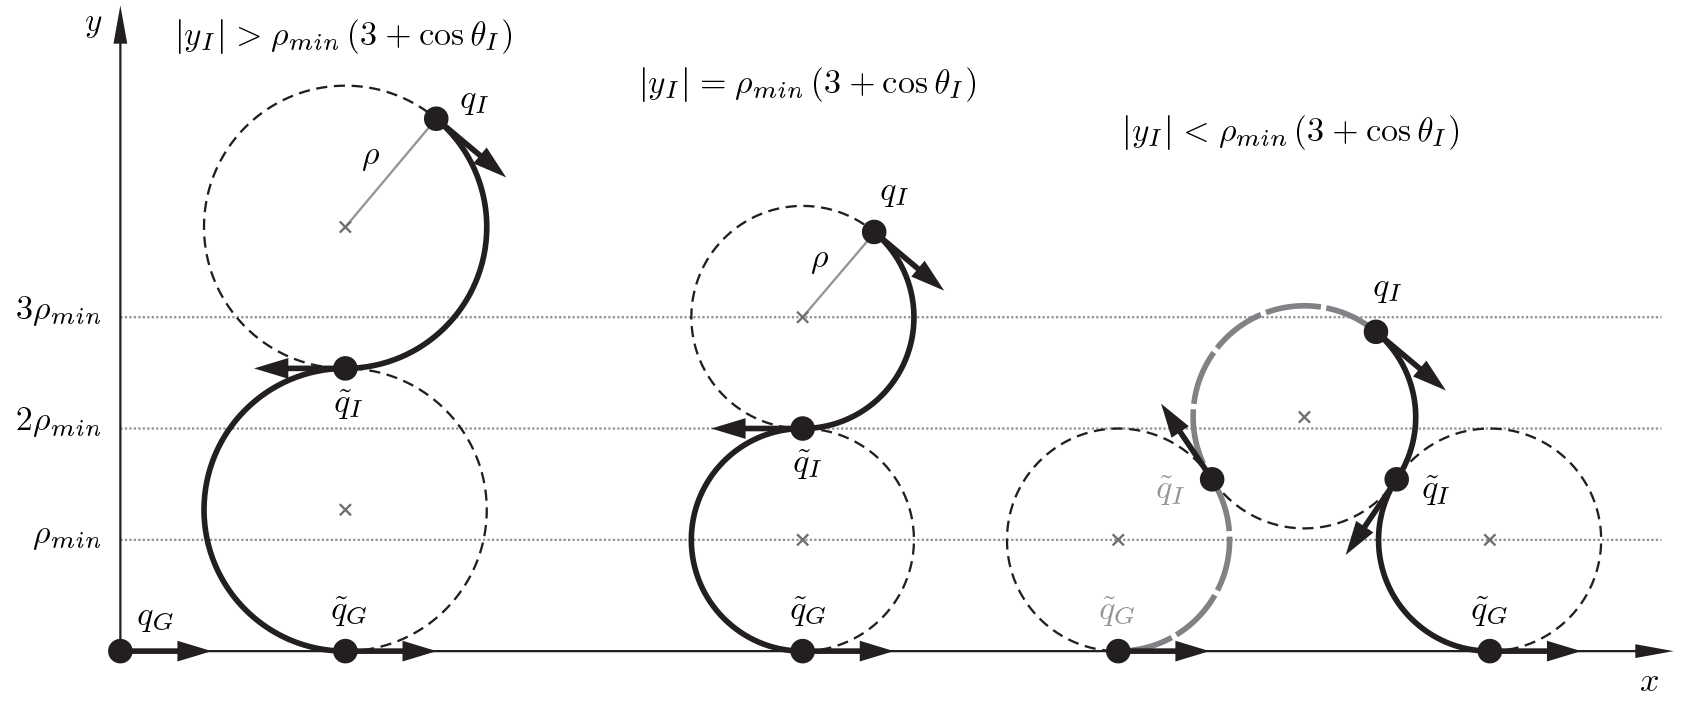
\includegraphics[width=130mm, keepaspectratio]{figures/cc_S.png}
\caption{A $c\overline{c}S$ algoritmus megold�sai k�l�nb�z� $y_{I}$ eset�n\cite{CCSTopologicalProp}} 
\label{fig:cc_S}
\end{figure}

Olyan esetekben, amikor a glob�lis p�ly�t tov�bb kellene bontanunk, �tv�ltunk a $c\overline{c}S$ algoritmusra, mely a topol�giai felt�telt teljes�ti. Ez az algoritmus a C*CS algoritmus egy m�dos�tott v�ltozata, mely csak egy megold�st ad egy konfigur�ci� p�rra. Az elj�r�s l�nyege, hogy az els� k�t k�r sugara minim�lis �s megegyez�, de ellent�tes el�jel�, teh�t a m�sik ir�nyba kell forgassuk a korm�nyt. A komplementer jel�l�s jelzi az el�jel v�ltoz�s�t. Ahogy \aref{fig:cc_S} �br�n l�that�, ha $q_{I}$ t�l k�zel van a $q_{G}$ egyenes�hez, akkor a k�r�k egym�s mellett elcs�sznak, �s k�t megold�st is adnak.

B�r a $c\overline{c}S$ egy megold�st ad, a v�grehajt�sakor t�bb lehets�ges megold�st is ``eldob''. A m�dszer implement�ci�j�t �gy k�sz�tettem el, hogy minden ilyen megold�st ellen�rizzen, ha esetleg a legr�videbb nem lenne v�grehajthat�, akkor v�lasszon m�sikat. Jogosan felmer�lhet a k�rd�s, hogy ha ez az algoritmus minden esetben ny�jt megold�st, akkor mi�rt nem ezt haszn�ljuk a C*CS helyett? B�r val�ban a $c\overline{c}S$ mindig haszn�lhat�, a C*CS t�bb lehets�ges megold�s k�z�l v�laszt, �gy a gyakorlatban term�szetesebb p�ly�kat ad eredm�ny�l.

%----------------------------------------------------------------------------
\section{Eredm�nyek}
%----------------------------------------------------------------------------
A feladatom megval�s�t�s�hoz rendelkez�sre �llt a C*CS algoritmus egy MATLAB scriptben meg�rt v�ltozata, ellenben ez csak demonstr�ci�s c�lokat szolg�lt, a feladatot lassan hajtotta v�gre, val�sz�n�leg az interpret�lt m�k�d�s k�vetkezt�ben, ez�rt v�lt sz�ks�gess� egy C++ implement�ci�.

\begin{figure}[H]
\centering
\includegraphics[height=60mm, keepaspectratio]{figures/frame3.png}
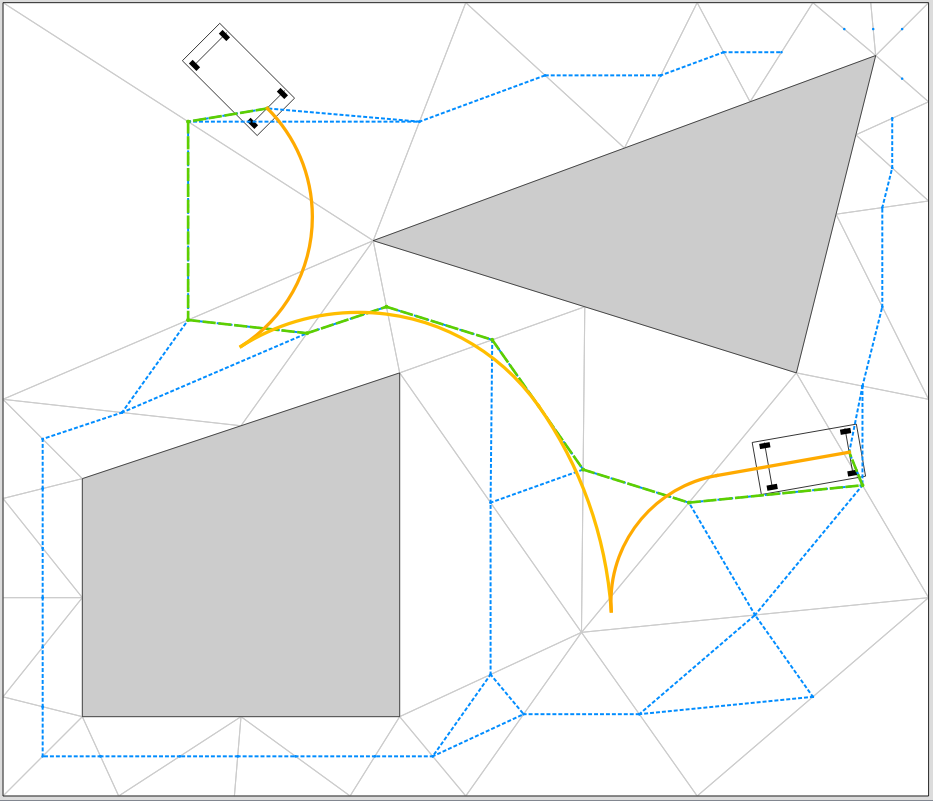
\includegraphics[height=60mm, keepaspectratio]{figures/frame6.png}
\caption{A C*CS algoritmus megold�sa k�l�nf�le k�rnyezetekben} 
\label{fig:ccssolutions}
\end{figure}

%TODO ide k�ne p�r m�r�s, hogy ne csak a leveg�be besz�ljek
\subsection{M�r�sek}
Pontos m�r�seket nem v�gezt�nk, de nagys�grendileg sz�zszoros gyorsul�st siker�lt el�rn�nk, �s a legbonyolultabb k�rnyezetben is egy m�sodpercen bel�l siker�lt megold�st tal�lnia az algoritmusnak\footnote{Intel Core 2 Duo E8400 @ 3.0GHz, 4GB RAM}. Ez egy igen nagy el�rel�p�s, �gy val�sz�n�, hogy egy kisebb teljes�tm�ny� be�gyazott sz�m�t�g�pen is elfogadhat� id�n bel�l v�gez.

\subsection{Fejleszt�si lehet�s�gek}
A fejleszt�s sor�n odafigyeltem, hogy hol lehetne gyors�tani, m�dos�tani a m�k�d�sen. Ahol ez egyszer�en megval�s�that� volt, ott ezeket megtettem, de maradtak tov�bbi fejleszt�si lehet�s�gek is a programban, p�ld�ul sz�mos helyen lehetne a fut�st p�rhuzamos�tani.

Az esetek nagy t�bbs�g�ben a celladekompoz�ci�s elj�r�ssal tervezett glob�lis p�lya j� eredm�nnyel szolg�l, de n�h�ny speci�lis esetben -- ilyen p�ld�ul k�t sz�k mer�leges folyos� tal�lkoz�sa, nem tal�lhat� megold�s. R�szben hasonl� probl�ma mikor a c�lkonfigur�ci� �s az utols� szakasz ir�nya jelent�sen elt�r -- ilyen probl�ma mer�l fel a p�rhuzamos parkol�s eset�n is. Ezek elker�l�s�re egy m�sik glob�lis tervez�t kell haszn�lnunk.

%----------------------------------------------------------------------------
\section{�j glob�lis tervez�}
%----------------------------------------------------------------------------
A fejleszt�s sor�n a fentebb felsorolt probl�m�k miatt a glob�lis tervez�t lecser�ltem az RTR nev� algoritmusra. Ez is Kiss Domokos munk�ja \cite{DomiRTR}, az implement�ci�j�t Nagy �kos v�gezte el \cite{Akos}. Ez egy, a szakirodalomban sz�les k�rben haszn�lt RRT (Rapidly Exploring Random Trees) m�dszeren alapul� p�lyatervez�si elj�r�s.

\subsection{RRT}
A glob�lis tervez�k sok esetben topologikus gr�fokat (speci�lis esetben f�kat) haszn�lnak a konfigur�ci�s t�r strukt�r�j�nak le�r�s�hoz \cite{kavraki96prm}. A szakirodalomban egyik leggyakrabban haszn�lt ilyen algoritmus a \emph{Rapidly Exploring Random Trees} \cite{LaValle}. Ennek a l�nyege, hogy a kezdeti konfigur�ci�b�l egy f�t �p�t�nk a szabadon bej�rhat� konfigur�ci�s t�rben. A fa csom�pontjaiban konfigur�ci�k tal�lhat�ak, �s a fa terjeszt�s�t �gy ir�ny�tjuk, hogy a k�v�nt c�lkonfigur�ci� fel� tartson. Ha a fa t�nylegesen el�ri a c�lkonfigur�ci�t, akkor az utat a kezdeti konfigur�ci�b�l a c�lkonfigur�ci�ba m�r k�nnyed�n megkaphatjuk.

\begin{figure}[H]
\centering
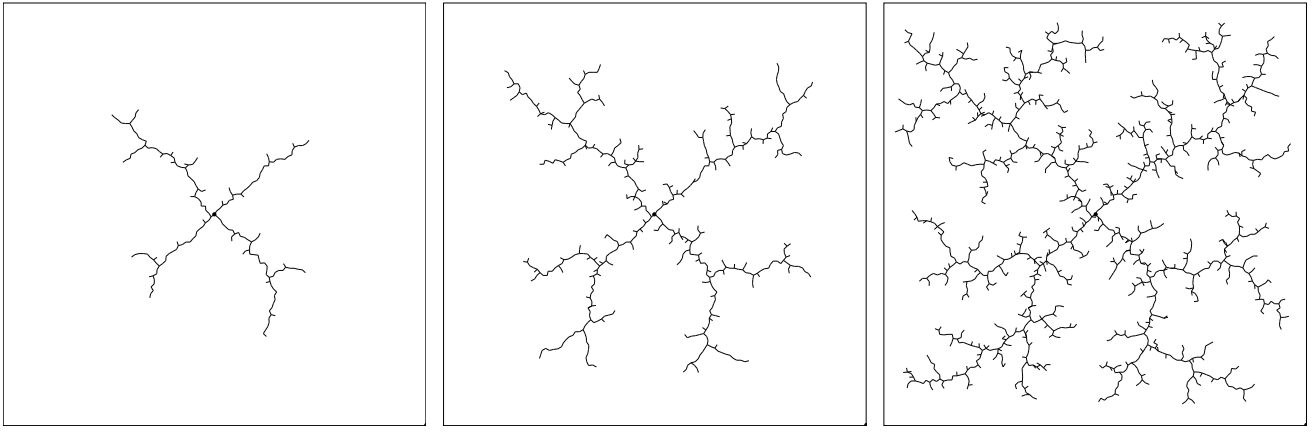
\includegraphics[width=130mm, keepaspectratio]{figures/RRT.png}
\caption{Az RRT algoritmus h�rom k�l�nb�z� iter�ci�n�l \cite{LaValle}.} 
\label{fig:RRT}
\end{figure}

\subsection{RTR}
Az \emph{Rotate-Translate-Rotate} algoritmus a fentebb l�tott RRT algoritmus egy m�dos�tott v�ltozata. Els�dlegesen differenci�lis robotok sz�m�ra tervez egyenes szakaszokb�l �s egy helyben fordul�sokb�l �ll� p�ly�t, de j� alapot szolg�ltat a C*CS algoritmushoz is. Nev�t a benne haszn�lt mozg�si primit�vekr�l kapta, azaz a $R$, mint fordul�s, a $T$ pedig az egyenesen halad�st jel�li. Az RRT algoritmust�l elt�r�en itt az algoritmus k�t f�t �p�t, egyet a kezd�, egyet pedig a c�lkonfigur�ci�b�l. M�sik fontos k�l�nbs�g, hogy �tk�z�s eset�n a p�ly�t minden ir�nyba tov�bbterjeszti, �gy n�velve a megold�s megtal�l�s�nak lehet�s�g�t.

\begin{figure}[b]
\centering
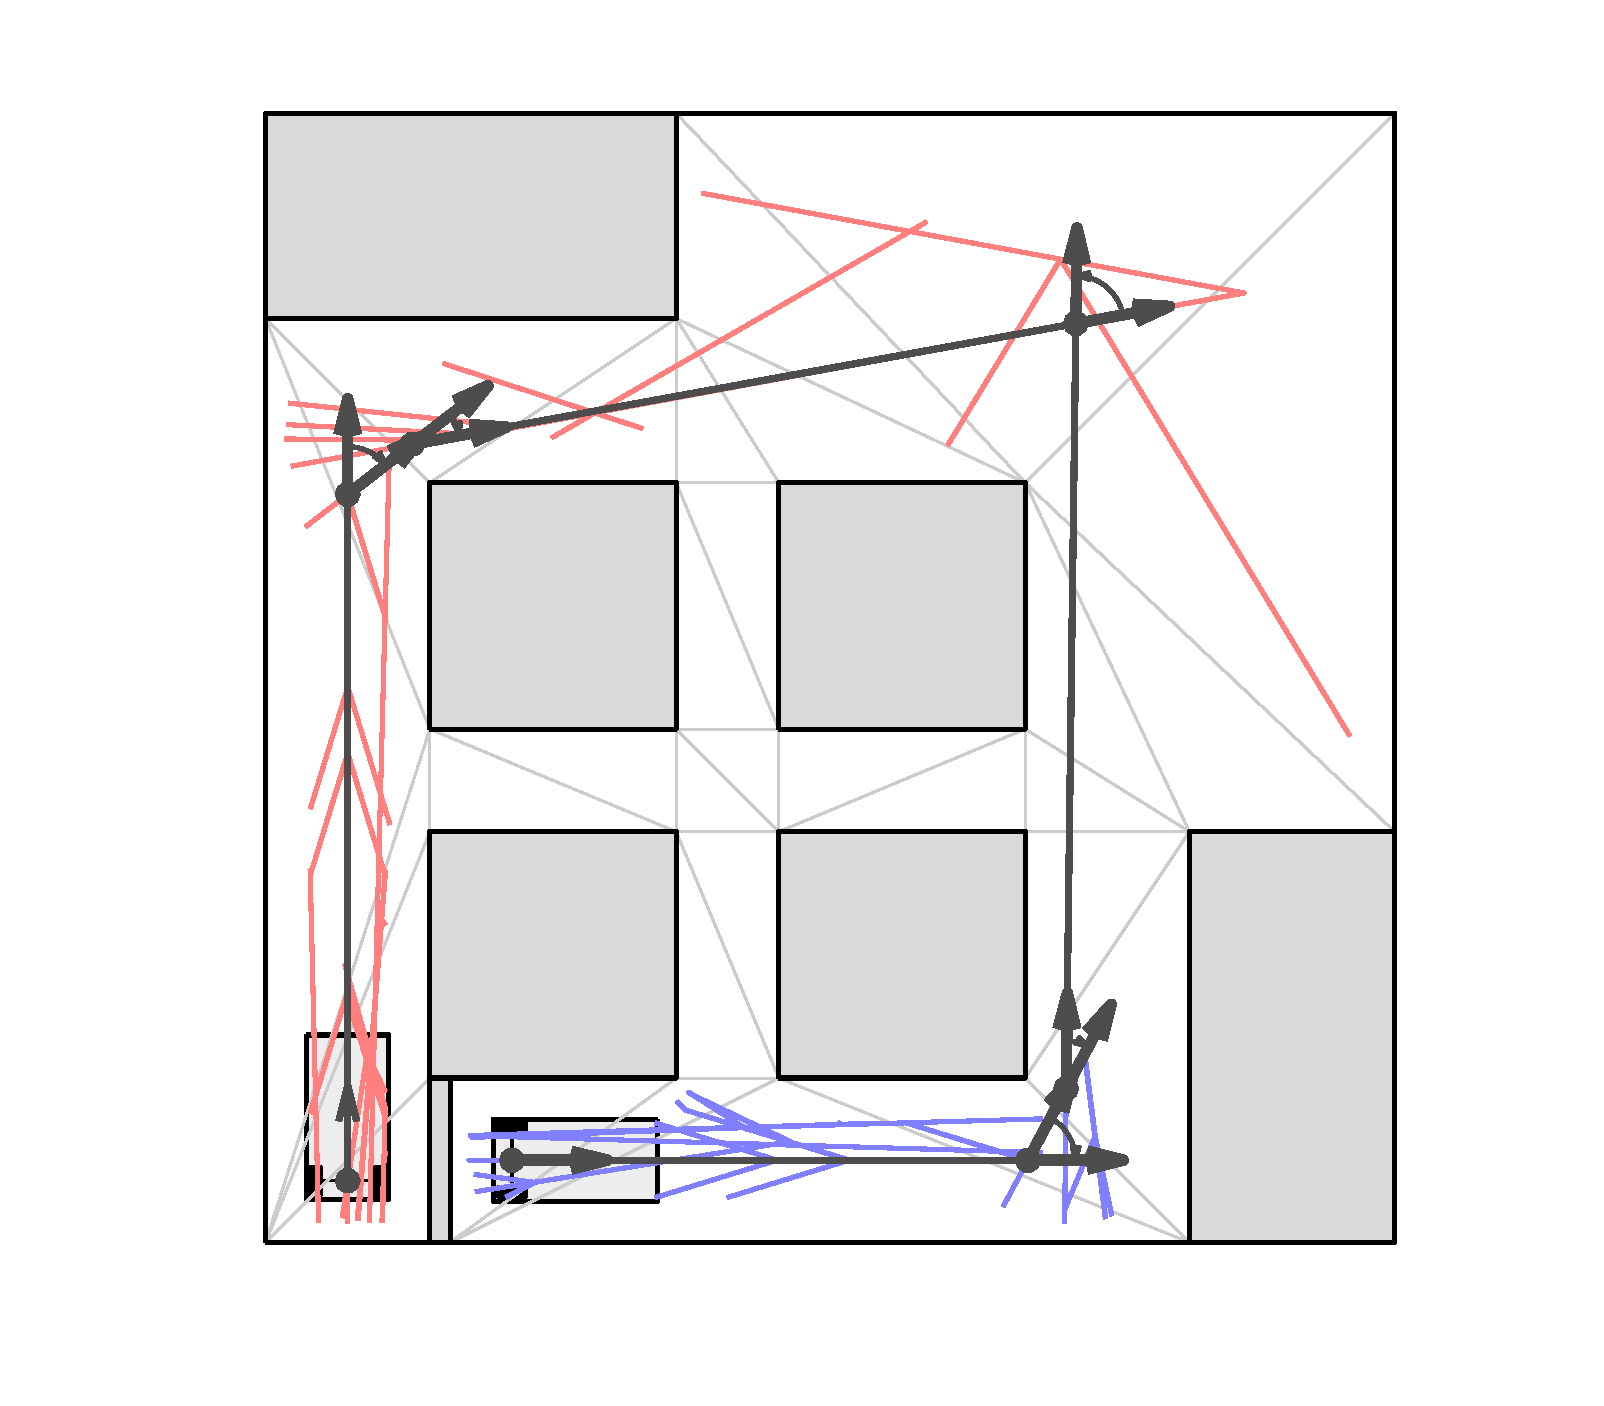
\includegraphics[width=110mm, keepaspectratio]{figures/rtr_path2.pdf}
\caption{Az RTR algoritmus; piros a kezd�, k�k a c�lkonfigur�ci�b�l ind�tott fa. \cite{Akos}}
\label{fig:rtr_path2}
\end{figure}

Ez az algoritmus az�rt el�ny�s, mert a celladekompoz�ci�s elj�r�s hib�j�t kik�sz�b�li. Teh�t k�t sz�k folyos� tal�lkoz�s�n�l csak akkor ad megold�st, ha van hely az elfordul�sra. Mivel a keres�s sor�n k�t f�t �p�t, �gy a p�rhuzamos parkol�s eset�n is seg�ti a megold�s megtal�l�s�t.
%----------------------------------------------------------------------------
\chapter{A C*CS, \boldmath{$c\overline{c}S$} algoritmus} \label{chapter:CCS}
%----------------------------------------------------------------------------
A C*CS �s a $c\overline{c}S$ algoritmus Kiss Domokos munk�ja \cite{CCSTopologicalProp}. Az algoritmusok els�dlegesen aut�szer� robotok sz�m�ra terveznek p�ly�t, de az �gy tervezett p�lya egy differenci�lis robot sz�m�ra is v�grehajthat�. Feladatunk az algoritmus implement�l�sa volt C++ nyelven, majd annak tesztel�se szimul�ci�s, illetve val�s k�rnyezetben.
A fejezetet az algoritmus ismertet�s�vel kezdj�k, majd kit�r�nk az implement�ci�s probl�m�kra, �s az el�rt eredm�nyekre.

%----------------------------------------------------------------------------
\section{Reeds-Shepp lok�lis p�ly�k}
%----------------------------------------------------------------------------
Az anholonom rendszerek ir�ny�t�sa akad�lyokt�l mentes k�rnyezetben is egy igen bonyolult feladat. Sok esetben nem adhat� meg �ltal�nos algoritmus, csak n�h�ny speci�lis rendszer eset�n. Szerencs�re ilyen rendszerek k�z� tartoznak a differenci�lis robotok, az aut�szer� robotok, amelyek csak el�re mozoghatnak (Dubins aut�), �s azok amelyek el�re �s h�tra is k�pesek mozogni.

\begin{figure}[H]
\centering
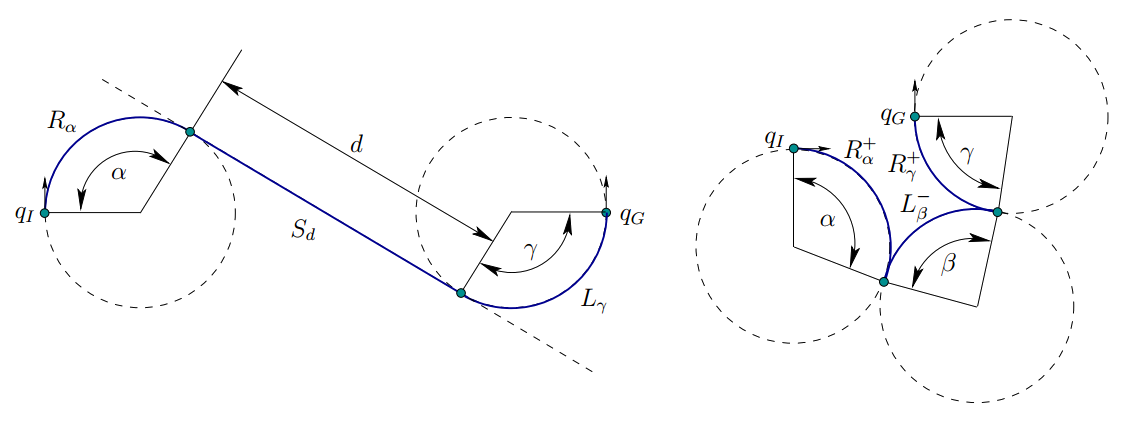
\includegraphics[width=130mm, keepaspectratio]{figures/dubins-reeds-shepp.png}
\caption{Dubins �s Reeds-Shepp megold�sok \cite{LaValle2}} 
\label{fig:reeds_shepp}
\end{figure}

\par
Az ut�bbi t�pus� robotokat h�vjuk Reeds-Shepp aut�knak, melyekn�l bizony�tott, hogy b�rmely kezd�- �s c�lkonfigur�ci� k�zt a legr�videbb utat megtal�lhatjuk 48 lehets�ges megold�s k�z�l, amelyb�l kett� l�that� \aref{fig:reeds_shepp} �br�n. Ezek a megold�sok maximum �t egyenes vagy k�r�v kombin�ci�j�b�l �llhatnak, �s a p�ly�k maximum k�t cs�csot tartalmazhatnak, azaz ennyiszer lehet ir�nyt v�ltoztatni a v�grehajt�s k�zben \cite{ReedsShepp}. A megold�sok sz�ma egy�b megk�t�sek �r�n tov�bb cs�kkenthet�.

\par
Mint l�that� akad�lyokt�l mentes k�rnyezetben tal�lhatunk optim�lis �tvonalat, de ennek h�tr�nya, hogy mindig minim�lis sugar� p�ly�kat felt�telez, mely egy val�s esetben nem �letszer�, illetve a p�ly�k lehetnek igen bonyolultak is. De ha elvetj�k az optimalit�s ig�ny�t, amit egy�bk�nt is meg kell tenn�nk, ha egy glob�lis tervez� r�szek�nt alkalmazzuk a m�dszert, akkor a lehets�ges megold�sokon jelent�s m�rt�kben egyszer�s�thet�nk. 

%----------------------------------------------------------------------------
\section{C*CS lok�lis p�ly�k}\label{CCSlocal}
%----------------------------------------------------------------------------
A lok�lis tervez�k b�rmely kezd�- �s c�lkonfigur�ci� p�ros eset�n megold�st kell ny�jtsanak, de megfelel� koordin�ta-rendszer v�laszt�s�val egyszer�s�thet�nk a sz�m�t�sokon. Tegy�k fel hogy egy ilyen v�laszt�s mellett ad�dott $q_{I} = (x_{I},y_{I},\theta_{I})$ kezd� �s $q_{G} = (0,0,0)$ c�lkonfigur�ci�. Ha eltekint�nk a minim�lis fordul�si sug�r korl�toz�s�t�l, �s feltessz�k, hogy $\theta_{I} \neq 0$, akkor k�nnyen bel�that�, hogy egy k�r �s egy egyenes seg�ts�g�vel el�rhet� a c�lkonfigur�ci�. El�sz�r egy �rint� k�r�n elfordulunk a $\tilde{q_{G}} = (\tilde{x_{G}},0,0)$ k�ztes c�lkonfigur�ci�ba, majd egy egyenes ment�n v�gighaladunk a c�lig. Az ehhez tartoz� k�r sugar�t a k�vetkez� egyenlet seg�ts�g�vel sz�m�thatjuk:
\begin{align}\label{eq:middleRadius}
\rho_{I,\tilde{G}} = \frac{y_{I}}{1 - \cos \theta_{I}}
\end{align}

\par
Ha a kiad�d� sug�r kisebb mint a minim�lisan megengedett ($|\rho_{I,\tilde{G}}| < \rho_{min}$), vagy igaz, hogy $\theta_{I} = 0$, akkor egy egyenes vagy egy k�r seg�ts�g�vel egy k�ztes kezd�konfigur�ci�ba ($\tilde{q_{I}} = (\tilde{x_{I}},\tilde{y_{I}},\tilde{\theta_{I}})$) kell eljutnunk, ahol biztos�tott, hogy $\tilde{\theta_{I}} \neq 0$ �s, hogy $\rho_{\tilde{I},\tilde{G}} \geq \rho_{min}$. Megjegyzend�, hogy az els� szakasz nem lehet egyenes, ha $\theta_{I} = 0$, $\theta_{I} = \pi$ vagy $|y_{I}| < 2\rho_{min}$. Bizony�tott, hogy $\tilde{q_{I}}$ megv�laszt�sa v�gtelen sokf�lek�ppen lehets�ges \cite{CCSTopologicalProp}. 

\par
Hogy egyszer�s�ts�k a szakaszok jel�l�s�t, a tov�bbiakban az egyes szakaszokra $S$ �s $C$ bet�k seg�ts�g�vel hivatkozunk. Az el�z�ek alapj�n egy konfigur�ci� p�rba $SCS$, vagy  $CCS$ seg�ts�g�vel eljuthatunk. K�nnyen bel�that�, hogy ha egy $C$ eset�n a sug�rral a v�gtelenbe tartunk, akkor a kiv�lasztott szakaszunk az egyeneshez tart. Az olyan speci�lis k�r�veket, amelyek sugara v�gtelen is lehet, $C^{*}$-gal jel�lj�k. Innen a m�dszer neve a $C^{*}CS$.

%----------------------------------------------------------------------------
\section{C*CS approxim�ci�s m�dszer}
%----------------------------------------------------------------------------
Az �ltalunk haszn�lt algoritmus egy approxim�ci�s m�dszert alkot, mely egy el�zetes glob�lis p�ly�t rekurz�v m�don felbont kisebb szakaszokra, majd ezekre pr�b�l illeszteni egy-egy fentebb bemutatott C*CS p�ly�t.\footnote{B�r a lok�lis tervez� algoritmus neve a C*CS, de a v�geredm�nyben kialakult p�lya �sszess�g�ben is k�r�k �s egyenesek kombin�ci�j�b�l �ll, �gy ez a n�v r�ragadt az approxim�ci�s m�dszerre is. A k�s�bbiekben, ahol ez f�lre�rt�sre adhat okot, ott ezt k�l�n tiszt�zzuk.} A v�geredm�ny�l elk�sz�lt, az algoritmus �ltal visszaadott p�lya aut�szer� robotok sz�m�ra k�nnyed�n lek�vethet�, mivel els�dlegesen ezek sz�m�ra lett kialak�tva. Ennek ellen�re a megold�st term�szetesen egy differenci�lis robot is k�pes lek�vetni, mivel az nem rendelkezik korl�toz�ssal a fordul� k�r sugar�t illet�en.

%----------------------------------------------------------------------------
\subsection{Glob�lis tervez�}\label{sect:CCSGlobal}
%----------------------------------------------------------------------------
Az el�zetes p�lya b�rmilyen glob�lis tervez� eredm�nye lehet. Els�dleges c�lja egy mank� ny�jt�sa a k�s�bbi tervez� sz�m�ra. A v�gs� megold�snak nem felt�tele, hogy az el�zetes p�lya ak�r egyetlen pontj�t is tartalmazza.

\par
Mi erre a c�lra egy celladekompoz�ci�n alapul� algoritmust haszn�ltunk. Ez az elj�r�s a k�rnyezetet h�romsz�gekre bontja, majd ezeknek a h�romsz�geknek az oldalfelez� pontjait �sszek�tve gr�fot alkot. Ebbe besz�rja a kezd�- �s c�lkonfigur�ci�t, majd ezeket �sszek�ti a legk�zelebb �ll� n�h�ny ponttal. Az �leket a pontok egym�st�l val� t�vols�g�val s�lyozzuk, majd ebben a gr�fban a Dijkstra-algoritmus \cite{BFS} seg�ts�g�vel megkeress�k a legr�videbb utat.

\begin{figure}
	\centering
	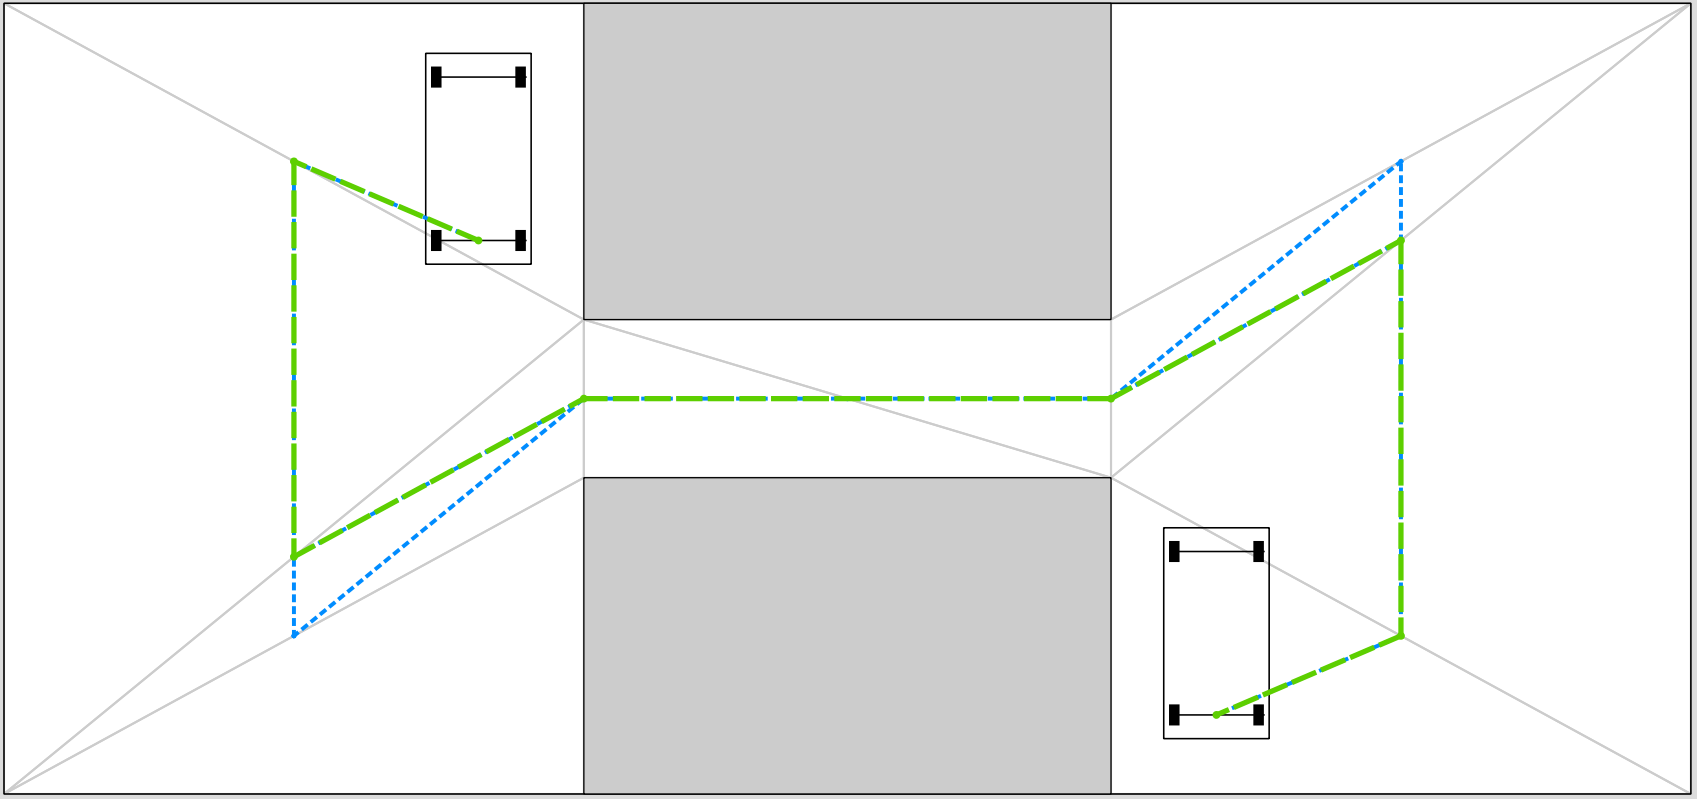
\includegraphics[width=130mm, keepaspectratio]{figures/ccs_prepath.png}
	\caption{Glob�lis tervez�: cella dekompoz�ci�, gr�f k�sz�t�s, �tvonal keres�s} 
	\label{fig:ccs_triang}
\end{figure}

Ennek a megold�snak az el�nye, hogy a szabad ter�let k�zep�n alkot p�ly�t, �gy ha az aut� ezt a p�ly�t k�veti, akkor b�rmilyen ir�ny� man�verez�sre lesz lehet�s�ge, ha a p�lya ezt megengedi. Tov�bbi el�nye, hogy ez egy kombinatorikus elj�r�s, �gy v�ges id�n bel�l k�pes megmondani, hogy l�tezik-e megold�s. Az elj�r�s egyik f� hib�ja, hogy a h�romsz�gel�s miatt, csak soksz�gekkel le�rhat� akad�lyokkal k�pes dolgozni, �s m�g ebben a form�j�ban nem veszi figyelembe az aut� kiterjed�s�t. Ezen k�nnyen lehet seg�teni, ha figyelembe vessz�k az oldalfelez� pontok k�z�tti szakaszok t�vols�g�t az akad�lyokt�l, �s ha a p�lya- �s az akad�ly�l t�l k�zel vannak egym�shoz, akkor t�r�lj�k az �lt a gr�fb�l. Sajnos az elj�r�s negat�vumokkal is b�r, amir�l a fejezet v�g�n m�g sz�t ejt�nk.

%----------------------------------------------------------------------------
\subsection{Lok�lis tervez� alkalmaz�sa}
%----------------------------------------------------------------------------
Ha a glob�lis tervez� tudott visszaadni megold�st, akkor az algoritmus tov�bb folytat�dik a k�vetkez�k�ppen: Az el�zetes p�lya k�t konfigur�ci�j�t v�lasztjuk ki, �s a fentebb eml�tett C*CS p�ly�kat keres�nk k�zt�k. Az elj�r�s el�sz�r a p�lya k�t v�gpontja k�zt keres �tvonalat, ami egyszer� esetekben ak�r r�gt�n megold�sra is vezethet, felgyors�tva az algoritmus m�k�d�s�t. Ha ez a keres�s nem j�rt sikerrel, akkor az el�zetes p�ly�t megfelezi az algoritmus, �s az els� konfigur�ci� valamint az �j c�lkonfigur�ci� k�zt keres megold�st. Ezt eg�szen addig ism�tli, m�g van k�ztes konfigur�ci�s pont, ha elfogyott, tov�bbi pontokat illeszt a p�ly�ba.

\par
Az el�z�ekben eml�tett�k, hogy a C*CS v�gtelen sok megold�st ny�jt. Lok�lis esetben ez nem el�ny�s tulajdons�g, de akad�lyok jelenl�t�ben m�r el�nyk�nt tekinthet�nk r�, mivel �gy sokkal nagyobb val�sz�n�s�ggel tal�lhatunk v�grehajthat� p�ly�t. Term�szetesen az �sszes megold�st nincs lehet�s�g�nk kipr�b�lni, �gy ezt a probl�m�t valamilyen mintav�telez� elj�r�ssal kell megoldanunk.

\begin{figure}[H]
\centering
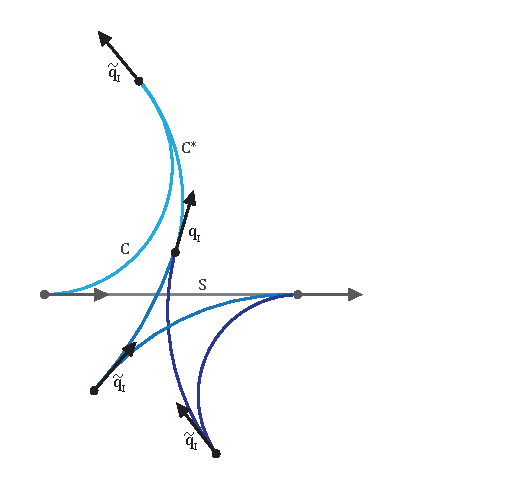
\includegraphics[width=75mm, keepaspectratio]{figures/CCS.pdf}
\caption{$q_{\tilde{I}}$ megv�laszt�sa } 
\label{fig:infCCS}
\end{figure}

\par
A v�gtelen sok megold�st a $\tilde{q_{I}}$ kiv�laszt�s�nak szabads�ga okozza. Erre egy p�lda l�that� \aref{fig:infCCS} �br�n. Ez�rt az algoritmus �sszegy�jti azokat a konfigur�ci�kat, melyeket a $q_{I}$ konfigur�ci�b�l �tk�z�s n�lk�l el�rhet�nk. Ehhez a k�rnyezetet fel kell osszuk egys�gnyi t�vols�gokra, mivel �gy v�ges sok lehet�s�get kapunk. A kisz�m�t�s ideje term�szetesen f�gg a v�lasztott t�vols�gegys�gt�l �s a k�rnyezet m�ret�t�l. Az eredm�nyek azt mutatj�k, hogy a teljes algoritmus fut�s�nak ez a leghosszabb r�sze, ami nem meglep�, mivel a k�r�vek kisz�m�t�sa komplex m�velet, �s ezt egy adott pont eset�n a robot test�nek minden cs�cs�ra ki kell sz�moljuk, hogy �tk�z�st tudjunk detekt�lni. A m�velet hat�konys�g�n t�bb m�don lehet jav�tani, p�ld�ul nagyobb t�vols�gegys�g megv�laszt�s�val. M�sik jav�t�si lehet�s�g, ha el�re elk�sz�t�nk egy foglalts�gi m�trixot, ami megmondja az adott pont akad�lyon be�l van-e, �gy ezekre a pontokra nem kell a sz�m�t�st elv�gezni. Mivel az �gy kapott k�r�vek egy adott kezd�konfigur�ci�hoz tartoznak, tov�bbi jav�t�si lehet�s�g lehet, ha az approxim�ci�s l�p�sben ink�bb a c�lkonfigur�ci� pontj�t mozgatjuk, �gy nem kell �jra �s �jra kisz�molni a k�r�ven el�rhet� sokas�got.

\begin{figure}[H]
\centering
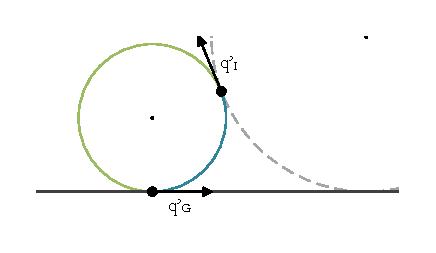
\includegraphics[width=90mm, keepaspectratio]{figures/CS.pdf}
\caption{K�z�ps� k�r�v sz�m�t�sa �rint� k�rrel} 
\label{fig:erintoKor}
\end{figure}

\par
Az algoritmus tov�bbi r�sz�ben \aref{CCSlocal} pontban l�tott m�don, a h�tral�v� k�r�v, �s egyenes szakasz kisz�m�t�sa a feladat. Egy ir�ny�tott k�r eset�n ez k�t lehets�ges p�ly�t jelent, amint az l�that� \aref{fig:erintoKor} �br�n. Ezek ut�n nem el�g csak a k�r�vek v�grehajthat�s�g�t ellen�rizn�nk, hanem meg kell n�zz�k ezt a h�tral�v� egyenes szakaszokra is. Ugyan a glob�lis p�lya tervez�sekor ellen�rizt�k ezeket, de az �rint� k�r�k keres�sekor nem volt felt�tel, hogy az �rint�si pontok ezeken a szakaszokon bel�l helyezkedjenek el, ez�rt ellen�rizn�nk kell a teljes szakaszon a v�grehajthat�s�got.

\par
V�g�l az �gy keletkez� v�grehajthat� p�ly�k sokas�ga k�z�l ki kell v�lasztanunk egyet. Ezt t�bbf�lek�ppen megtehetj�k. Tal�n a legk�zenfekv�bb a legr�videbb megold�s kikeres�se �s beilleszt�se az el�zetes p�ly�ba. Itt �rdemes megeml�teni, hogy a v�geredm�ny akkor fog igaz�n hasonl�tani a val�s�ghoz, ha lecs�kkentj�k a tolat�sok sz�m�t, mivel az emberek nagy t�bbs�ge nem szeret tolatva k�zlekedni. Hogy ezt megtehess�k, az algoritmus opcion�lisan elfogad egy s�lyt�nyez�t, mellyel a tolat� szakaszok ``hossz�t'' tudjuk megn�velni.

\begin{figure}[H]
\centering
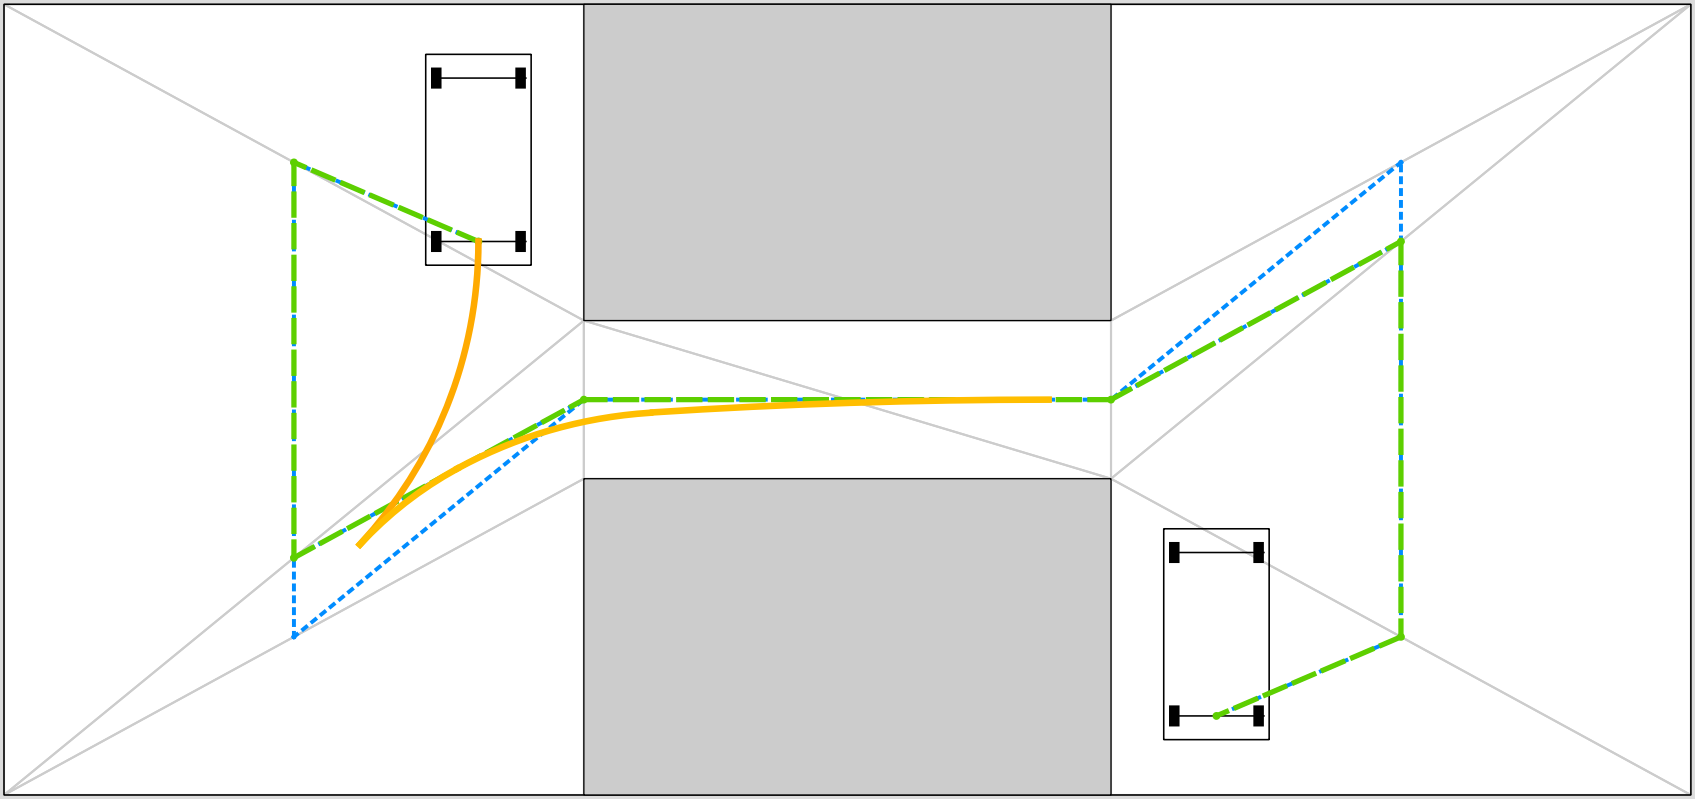
\includegraphics[width=130mm, keepaspectratio]{figures/ccs_middle.png}
\caption{A C*CS algoritmus m�k�d�s k�zben} 
\label{fig:CCSonline}
\end{figure}

%----------------------------------------------------------------------------
\section{\boldmath{$c\overline{c}S$}}
%----------------------------------------------------------------------------
Ha az el�z�ekben l�tottak nem vezetnek megold�sra, teh�t nincs olyan C*CS p�lya, mely v�grehajthat� lenne, akkor egy kisebb szakaszt kell v�lasztanunk a glob�lis p�ly�b�l. Ezt viszont nem tehetj�k meg v�gtelens�gig. Az egyik ok p�ld�ul az, hogy a glob�lis p�lya szakaszok nem bonthat�k t�bb r�szre, mert ha ki is v�lasztunk egy pontot a szakasz k�zep�r�l, akkor is ugyan arra az egyenesre pr�b�ln�nk meg �rint� k�r�ket tal�lni. Persze kereshet�nk k�l�nb�z� megold�sokat az �jabb konfigur�ci�k kiv�laszt�s�ra, de ezek a megold�sok �nmagukban nem elegend�ek. Valahogy biztos�tanunk kell azt, hogy az algoritmusunk konverg�ljon a megold�s fel�, amihez olyan lok�lis tervez�re van sz�ks�g�nk, mely teljes�ti a topol�giai felt�telt \cite{CCSTopologicalProp}. Ha ezt biztos�tani tudjuk, akkor az approxim�ci�s algoritmusunk teljes lesz. A teljess�g itt azt jelenti, hogy az algoritmus minden olyan esetben megold�ssal t�r vissza, mikor a glob�lis tervez� �rv�nyes p�ly�t ad vissza. Teh�t a k�r�vekkel val� k�zel�t�s nem cs�kkenti a megold�s l�tez�s�nek es�ly�t.

\begin{figure}[H]
\centering
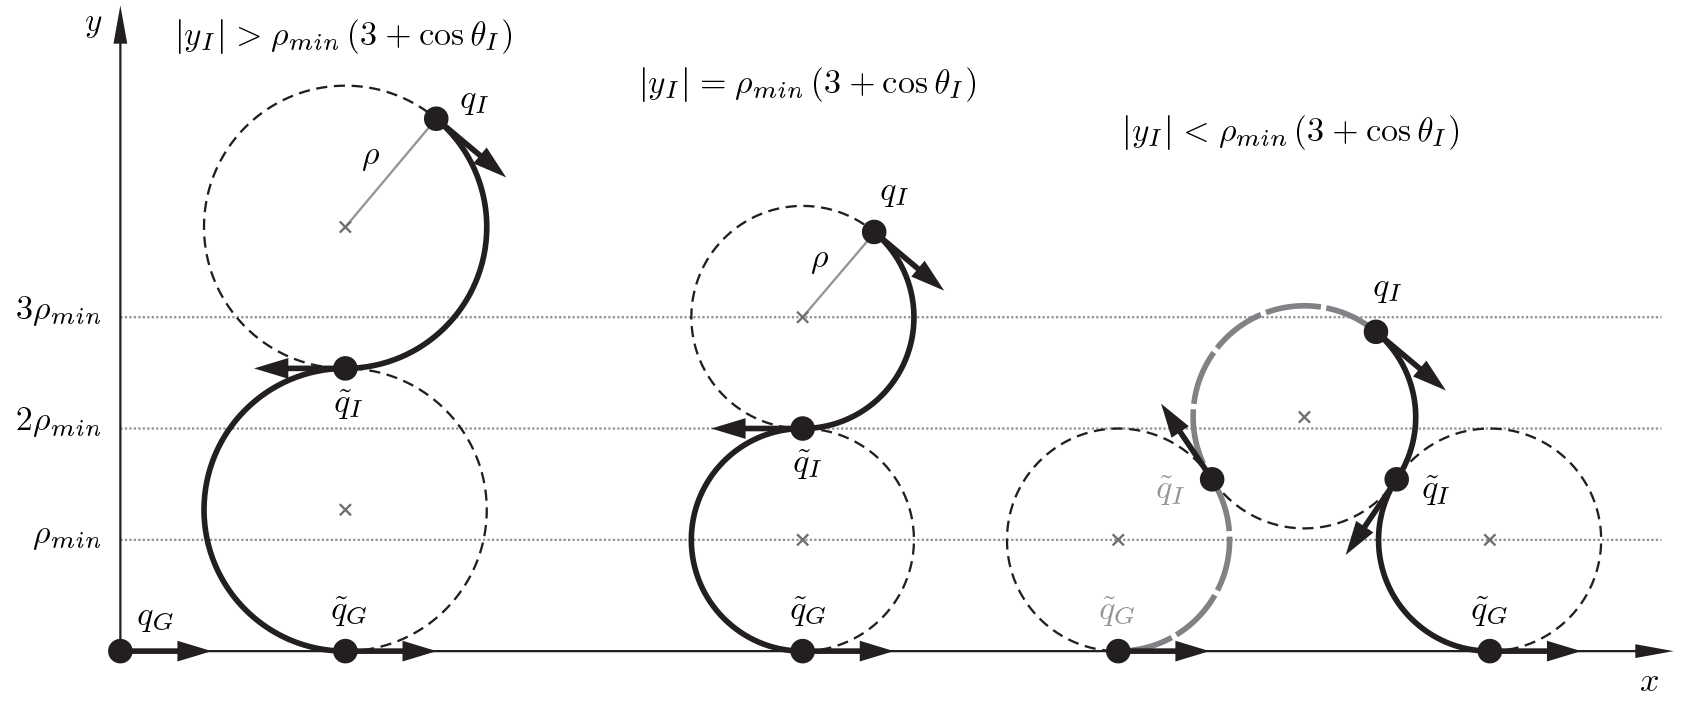
\includegraphics[width=130mm, keepaspectratio]{figures/cc_S.png}
\caption{A $c\overline{c}S$ algoritmus megold�sai k�l�nb�z� $y_{I}$ eset�n\cite{CCSTopologicalProp}} 
\label{fig:cc_S}
\end{figure}

\par
Olyan esetekben, amikor a glob�lis p�ly�t tov�bb kellene bontanunk, �tv�ltunk a $c\overline{c}S$ algoritmusra, mely a topol�giai felt�telt teljes�ti. Ez az algoritmus a C*CS algoritmus egy m�dos�tott v�ltozata, mely csak egy megold�st ad egy konfigur�ci� p�rra. Az elj�r�s l�nyege, hogy az els� k�t k�r sugara megegyez�, de ellent�tes el�jel�, teh�t a m�sik ir�nyba kell forgassuk a korm�nyt. A komplementer jel�l�s jelzi az el�jel v�ltoz�s�t. Ahogy \aref{fig:cc_S} �br�n l�that�, ha $q_{I}$ t�l k�zel van a $q_{G}$ egyenes�hez, akkor a k�r�k egym�s mellett elcs�sznak, �s k�t megold�st is adnak.

\par
B�r a $c\overline{c}S$ egy megold�st ad, a v�grehajt�sakor t�bb lehets�ges megold�st is ``eldob''. A m�dszer implement�ci�j�t �gy k�sz�tett�k el, hogy minden ilyen megold�st ellen�rizzen, ha esetleg a legr�videbb nem lenne v�grehajthat�, akkor v�lasszon m�sikat. Jogosan felmer�lhet a k�rd�s, hogy ha ez az algoritmus minden esetben ny�jt megold�st, akkor mi�rt nem ezt haszn�ljuk a C*CS helyett? B�r val�ban a $c\overline{c}S$ mindig haszn�lhat�, a C*CS t�bb lehets�ges megold�s k�z�l v�laszt, �gy a gyakorlatban term�szetesebb p�ly�kat ad eredm�ny�l.

%----------------------------------------------------------------------------
\section{Eredm�nyek}
%----------------------------------------------------------------------------
A tervez� algoritmus fut�sa k�zben nagy mennyis�g� lebeg�pontos sz�m�t�st v�gez, de ezen fel�l viszonylag nagy mem�riaig�ny� is, �s sok iter�ci�s szakasza van. Az algoritmus egy implement�lt v�ltozata rendelkez�sre �llt MATLAB script form�tumban, de ez els�dlegesen demonstr�ci�s c�lt szolg�lt. Ett�l a nyelvt�l azt v�rn�nk, hogy a lebeg�pontos sz�m�t�sokat gyorsan k�pes elv�gezni, de a feladatot rendk�v�l lassan hajtotta v�gre. Ennek els�dleges oka val�sz�n�leg az interpret�lt m�k�d�s. Az ilyen algoritmusokra nem ez a legalkalmasabb nyelv, ez�rt is mer�lt fel els�dlegesen egy g�pk�zeli nyelv haszn�lata. A legnagyobb tapasztalatunk a C++ nyelvvel kapcsolatban volt, �s grafikus sz�m�t�sok sor�n is ezt a nyelvet szokt�k haszn�lni a hat�konys�ga miatt.

\begin{figure}[H]
\centering
\includegraphics[height=60mm, keepaspectratio]{figures/frame3.png}
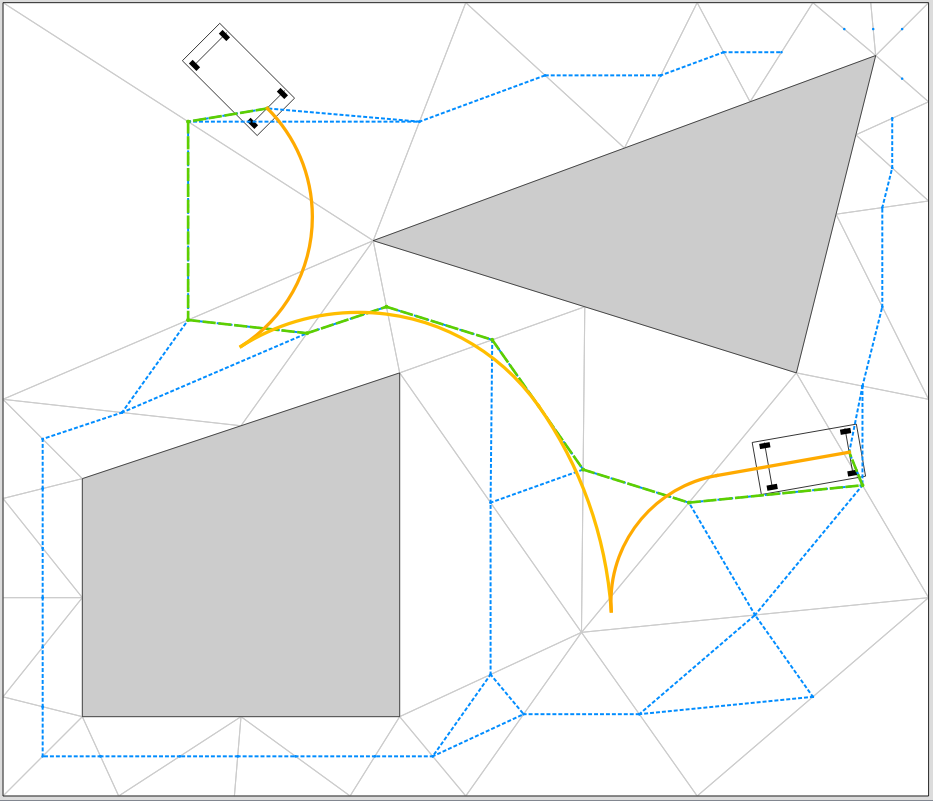
\includegraphics[height=60mm, keepaspectratio]{figures/frame6.png}
\caption{A C*CS algoritmus megold�sa k�l�nf�le k�rnyezetekben} 
\label{fig:ccssolutions}
\end{figure}

\par
Pontos m�r�seket nem v�gezt�nk, de nagys�grendileg sz�zszoros gyorsul�st siker�lt el�rn�nk, �s a legbonyolultabb k�rnyezetben is egy m�sodpercen bel�l siker�lt megold�st tal�lnia az algoritmusnak\footnote{Intel Core 2 Duo E8400 @ 3.0GHz, 4GB RAM}. Ez egy igen nagy el�rel�p�s, �gy val�sz�n�, hogy egy kisebb teljes�tm�ny� be�gyazott sz�m�t�g�pen is elfogadhat� id�n bel�l v�gez.

\par
A fejleszt�s sor�n odafigyelt�nk, hogy hol lehetne gyors�tani, m�dos�tani a m�k�d�sen. Ahol ez egyszer�en megval�s�that� volt, ott ezeket elv�gezt�k, de maradtak tov�bbi fejleszt�si lehet�s�gek is a programban.

\par
Az esetek nagy t�bbs�g�ben a celladekompoz�ci�s elj�r�ssal tervezett glob�lis p�lya j� eredm�nnyel szolg�l, de n�h�ny speci�lis esetben lehets�ges, hogy olyan p�ly�val t�r vissza, melyet egy aut�val k�ptelens�g lek�vetni. Ilyen eset p�ld�ul k�t, egym�sra mer�leges, aut� sz�less�g� folyos�, ahol az elfordul�sra nincs hely, de ezt a glob�lis tervez� nem veszi �szre. Egy m�sik probl�m�s eset a p�rhuzamos parkol�s, ahol b�r �gy t�nik v�grehajthat� lenne, de a glob�lis tervez�s sor�n kialakult konfigur�ci�k ezt nem teszik lehet�v�. A k�vetkez� fejezetben bemutatunk egy m�sik glob�lis tervez�t, mely ezeket a probl�m�kat megoldja.














%----------------------------------------------------------------------------
\chapter*{K�sz�netnyilv�n�t�s}\addcontentsline{toc}{chapter}{K�sz�netnyilv�n�t�s}
%----------------------------------------------------------------------------

Szeretn�nk k�sz�netet mondani Kiss Domokosnak a folyamatos konzult�ci�k�rt, tan�csai�rt �s ir�nymutat�sai�rt. 

%\listoffigures\addcontentsline{toc}{chapter}{�br�k jegyz�ke}
%\listoftables\addcontentsline{toc}{chapter}{T�bl�zatok jegyz�ke}

\bibliography{mybib}
\addcontentsline{toc}{chapter}{Irodalomjegyz�k}
\bibliographystyle{plain}

%----------------------------------------------------------------------------
\appendix
%----------------------------------------------------------------------------
\chapter*{F�ggel�k}\addcontentsline{toc}{chapter}{F�ggel�k}


\label{page:last}
\end{document}
